\documentclass[a4paper, 12pt]{report}
\usepackage{graphicx}
\usepackage{float}
\usepackage{listings}
\newcommand{\namesigdate}[2][5cm]{%
  \begin{tabular}{@{}p{#1}@{}}
    #2 \\[2\normalbaselineskip] \hrule \\[0pt]
    {\small \textit{Signature}}
  \end{tabular}
}

\linespread{1.3}
\lstdefinelanguage{JavaScript}{
  keywords={typeof, new, true, false, catch, function, return, null, catch, switch, var, if, in, while, do, else, case, break},
  %keywordstyle=\color{blue}\bfseries,
  ndkeywords={class, export, boolean, throw, implements, import, this},
  %ndkeywordstyle=\color{darkgray}\bfseries,
  %identifierstyle=\color{black},
  sensitive=false,
  comment=[l]{//},
  morecomment=[s]{/*}{*/},
  %commentstyle=\color{purple}\ttfamily,
  %stringstyle=\color{red}\ttfamily,
  morestring=[b]',
  morestring=[b]"
}

\begin{document}
\lstset{language=JavaScript, basicstyle=\footnotesize\ttfamily, tabsize=1, showstringspaces=false}
\begin{titlepage}
    \centering
    \vfill
    {\bfseries\Large
        Final Year Project Name\\
        2014\\
        \vskip2cm
        Fintan O'Hea\\
        109690999\\
    }    
    \vfill
    
\includegraphics[width=4cm]{ucc_crest.jpg} % also works with logo.pdf
    \vfill
    \vfill
\end{titlepage}

\clearpage

\begin{center}
\Large \textbf{B.Sc. Final Year Project Report \\
2014}
\end{center}
 %\vskip1.5cm
\begin{flushleft}
%\Large \textbf{Student Name:} Fintan O'Hea\\
%\textbf{Student ID:} 109690999\\
%\textbf{Supervisor:} Gavin Russell\\
%\textbf{Second Reader:} Humphrey Sorensen\\
\end{flushleft}
\begin{center}
\Large \textbf{Declaration of Originality}
\end{center}
In signing this declaration, you are confirming, in writing, that the submitted work is your own original work, unless clearly indicated otherwise, in which case, it has been fully and properly acknowledged. \\


\begin{description}
\item[I hereby declare that:]
\end{description}
\begin{itemize}
\item this is all my own work, unless clearly indicated otherwise, with full and proper accreditation;
\item with respect to my own work: none of it has been submitted at any educational institution contributing in any way towards an educational award;
\item with respect to another’s work: all text, diagrams, code, or ideas whether verbatim, paraphrased or otherwise modified or adapted, have been duly attributed to the source in a scholarly manner, whether from books, papers, lecture notes or any other students work, whether published or unpublished, electronically or in print.
\end{itemize}
\vskip1.5cm
\noindent \namesigdate{Fintan O'Hea}

\clearpage

\paragraph{}
\begin{center}
\Large \textbf{Acknowledgements}
\end{center}
A special thank you must go to my supervisor, Mr. Gavin Russell, for providing me with the opportunity to work on a project in which I have great interest and for his continued support, guidance and professionalism throughout the college year. I would also like to thank all the professionals with whom we met throughout the course of the project, your advice and suggestions have been invaluable.\\

\vskip1.5cm

\begin{center}
\Large \textbf{Abstract}
\end{center}
This projects main function is to develop a web application, with the purpose of creating a music station which users can interact with to determine the contents of the station playlist. The owner of the station creates the playlist for the station using music from their own personal library in the system consisting of their own personal uploads or music uploaded by other users.  \\
\clearpage

\tableofcontents
\clearpage

\chapter{Introduction}

\section{Introduction}
No matter where you are in the world or what culture you are in music plays a huge part. It has been part of culture for millennia dating back to our ancestors in Africa and is one of the most beloved human experiences. Music is present in almost every human event from weddings to funerals. The ambiance in a room can set by simply playing soft music in a restaurant or upbeat music at a party. \\

Music is used as inspiration, reminiscing, and celebrating. National anthems are sung before sporting events to hype up the players and crowd alike, hearing a certain song can return you to moments you didn’t even know you remembered, and a birthday is never celebrated without singing "Happy Birthday".  \\

Without music life is colourless. Everything is done to a tune and that has never been truer than now with a near limitless archive of music just a touch away using a smart phone. Each adventure requires an anthem, every moment needs a melody, and every life needs a soundtrack. \\%Carlos Santana once said; "music can change your molecular structure" and maybe he was right. If music changes our molecular structure what would we be without it? \\



\section{Motivation}
Currently there is a large number of people bewildered by the current means of listening to music. Despite all the advancements in technology there has been no real developments in how music is listened to. There is a larger amount of radio stations available due to websites such as last.fm, Grooveshark and 8tracks but they still follow the old ways of making set playlists and receiving zero listener feedback. \\

The distinct lack of flexibility in the current system means that social events are dominated by over priced DJ's that basically play all the same music and if anyone has a request they must make their way to the DJ and shout it in their ear. With music being an integral part of events the guests should be able to dictate what is being played. Developing a Juke Box style application would give this power to the people while also adding an extra dynamic to social events. \\

This application would also provide the perfect base for music enthusiasts and aspiring DJ's to enjoy their love in an entirely new way and practice their trade by learning which songs fit in which set lists while running a station session by receiving the listeners feedback. These users would also from discovering new music by listening to other users station sessions. 


\section{Aim of the Project}
This projects main function is to develop a web application, with the purpose of creating a music station which users can interact with to determine the contents of the stations playlist. The owner of the station creates the playlist for the station using music from their own personal library in the system consisting of their own personal uploads or music uploaded by other users which is part of a user-curated library and registered user can access.  \\

Overall, this application will allow users have more control over the music they listen to by voting for listed songs available in a given station. This vote will help determine the next track to be played by either being a reference for the station owner while they are deciding the next track or being part of a list of tracks where the next top voted track is selected to play.\\

Users will also be provided with an extensive collection of music consisting of all the music uploaded by the community using the application. Users will be able to browse this collection and create their own personal library’s with its contents, and with this personal library will be able to create live station sessions where users can either vote for the next song to be played or stream the playlist depending on what station type is created.

\section{Report Outline}
The report is split into several chapters, they are;
\begin{itemize}
\item \textbf{Introduction} - This chapter introduces the reader to the project problem and it's aim. 
\item \textbf{Background} - This chapter outlines the technologies used and a brief analysis of the applications already available.
\item \textbf{Design} - This chapter describes the overall design of the application, including requirements, architecture, navigation, screen designs and data storage choices.
\item \textbf{Implementation} - This chapter explains the implementation of some of the major components of the project.
\item \textbf{Testing and Evaluation} - This chapter covers the testing and evaluation of the application.
\item \textbf{Conclusion} - This chapter is the conclusion of the project, and a personal conclusion.
\item \textbf{Future} - This chapter focuses on the changes and inclusions of technologies that could be implemented in the future.
\end{itemize}
\textbf{Accompanying} this report is a CD containing the project code.


\clearpage
\chapter{Background}

\section{Relevant Technologies}
This section will list the technologies that were relevant to the project.

\subsection{Apache HTTP Server}
Apache is the web server that was used during the development of this project. Apache is the most popular server in the world and as of March 2014 was estimated to serve 39\% of all active websites and 52\% of active websites\cite{apache}.

\subsection{MySQL}
MySQL is an open-source relational database management system. It is used in many high-profile, large-scale websites including Wikipedia.com, Google, Facebook.com, Twitter.com and Youtube.com\cite{MySQL}

\subsection{PHP}
PHP is a server-side scripting language designed for web development. Some of the most popular websites use PHP such as Facebook.com, Twitter.com and Wikipedia.com. As of March 2014 81\% of websites use PHP\cite{php}. 

\subsection{JavaScript}
JavaScript is a dynamic computer programming language whose implementation allows client-side scripts to interact with the user, communicate asynchronously, and alter document content that is displayed\cite{javascript}.

\subsection{jQuery}
Jquery is a cross-platform JavaScript library which is used by over 80\% of the 10,000 most visited websites\cite{jquery}.

\subsection{jPlayer}
jPlayer is a cross-browser JavaScript library developed as a jQuery Plugin which facilitates the embedding of web based media\cite{jplayer}.

\section{Research}
The area of music based web applications is extremely broad so there was a lot of research done first to see what applications were already available and how they worked.

\subsection{Grooveshark}
Grooveshark\cite{grooveshark} is a rich Internet application designed in HTML5. It allows users to search and find music by song, artist, album, or through other users playlists. The service allows users to create and edit Playlists. Registered users can save playlists to an account, subscribe to other users’ Playlists, and share Playlists through e-mail, social media, StumbleUpon, Reddit or an embeddable widget. Users can listen to Genre Radio Stations of particular genres or they can populate their own station via their list of Current Songs. \\

Grooveshark ticks most of the boxes when looking for a solution to the problem. Users can browse a huge user-curated library of music and create their own personal libraries. With these libraries they can create playlists and broadcast them live for other users to access. While these playlists are being broadcast users can vote for any song available on Grooveshark that they would like to be played next. The live broadcasts lack the main functionality needed for this project which would allow users to only vote for songs in the playlist for the station and allow the next top voted song to be played automatically.

\subsection{8tracks}
8tracks\cite{8tracks} is an internet radio website revolving around the concept of streaming user curated playlists consisting of at least 8 tracks. Users can either browse the site and listen to playlists created by other users, and/or create their own playlists. Playlists can be discovered by selecting what mood they are in, genre, or by activity\\

Overall 8tracks did not offer much different from its competitors. The main feature that sets it apart from the others is that users can browse playlists by the mood/theme that they have been tagged with eg. Happy, Nostalgic or Summer, which allows users discover new music.
The main drawbacks to this service solving the problem at hand is the lack of flexibility and a lack of a user-curated library. Users create set playlists from music they either upload themselves on 8tracks or Soundcloud\cite{soundcloud} which is a service that allows users to upload, record, promote and share their originally-created sounds. Users also receive zero feedback from listeners apart from the number of times the playlist has been viewed. 

\subsection{Spotify}
Spotify\cite{Spotify} is a commercial music streaming service providing content from record labels. It provides a catalogue of over 20 million songs which can be search by artist, album, song name, label and genre. Due to providing the music from the record labels some artists have decided not to be available on Spotify, also some artists are missing in certain regions due to record label licensing restrictions. \\
Users can create and share playlists. These playlists can then be edited by the user or collaboratively with other users. Spotify also has a radio feature which creates a random playlist of songs chosen based on specific genres, decades and artists.\\

Yet again we see a service that offers great functionality needed to discover new music and allowing users add these to their own personal collections but offers no flexibility to the playlists that are created. 

\subsection{Pandora}
Pandora\cite{pandora} is a music streaming and automated music recommendation service. Users enter an artist, genre or composer and Pandora creates a radio station featuring that music and more like it. The user then provides positive or negative feedback for songs chosen by the service, which are taken into account when Pandora selects future songs. To comply with the requirements and protections offered by the DMCA, Pandora only serves users in the United States, New Zealand and Australia. \\

Pandora has been extremely popular for many years now but is essentially just a music recommender which is now highly limited due to its restriction to only the United States, New Zealand and Australia. 

\subsection{Research Conclusion}
After much research there appeared to be no current applications available that would fulfil the needs of the problem. There is a huge selection of services available for simply streaming music and publishing playlists but there is no flexibility offered and very little listener feedback.\\

Grooveshark appeared to be the service most like what was being searched for due to its user-curated archive of music, ability to create your own personal collections using either songs you have uploaded yourself or by others, publish playlists for other users to listen to, and allow others to provide suggestions for the next song to be played. 
The main drawback to Grooveshark however is that the next top voted song is not played automatically which means it still relies on the owner of the broadcast playlist to select the next song. Also listeners can suggest any song available from the entire Grooveshark library. Therefore it is susceptible to cyber attacks where a group of people can spam votes for unwanted songs.

\clearpage
\chapter{Design}

\section{High Level Requirements}
The user should be able to:
\begin{itemize}
\item Create an account.
\item Have a personal library containing their music.
\item Upload mp3 files from their own device to their library.
\item Browse a library containing music uploaded by other users.
\item Browse live stations being broadcast by other users.
\item Play music uploaded by other users.
\item Add music uploaded by other users to their own personal library. 
\item Create a playlist containing music from their own library.
\item Set whether users connected to the station can vote for the next song to be played.
\item Connect to other users stations.
\item Search music available while connected to other users stations.
\item Vote for a song to be added to the queue if they have permission to.
\item While listening to another station add the current song to their personal library.
\end{itemize}
 
 
\section{Detailed Requirements} 

\subsection{Features available to unregistered users}
Unregistered users will have limited privileges. They will only be able to connect to stations being broadcast at that moment and carry out the privileges given to them by the station permissions eg. upvoting/downvoting a song, streaming the station.

\subsection{Features available to registered users}
In order to access all the features of this web application users will be requested to create an account. Once they have done this users will then be able to;
\begin{itemize}
\item Create a personal library.
\item Edit their personal library.
\item Gain access to the user-curated library of music.
\item Create a station.
\item Edit existing stations they have created.
\item Delete existing stations they have created.
\item Connect to live stations being broadcast.
\end{itemize}

 
\subsection{Creating an account} 
Users will have the ability to create an account by filling out a form with the following stipulations : 
\begin{itemize}
\item Usernames may contain only digits, upper and lower case letters and underscores.
\item Emails must have a valid email format.
\item Passwords must be at least 6 characters long.
\item Passwords must contain.
\begin{itemize}
\item At least one upper case letter (A..Z)
\item At least one lower case letter (a..z)
\item At least one number (0..9)
\end{itemize}
\item The password and confirmation must match exactly.
\end{itemize}
By creating an account users gain certain privileges as opposed to being an unregistered user. 

\subsection{Creating a personal library} 
Once a user has created an account they will be able to add songs to their personal library. This can be done in one of three ways. The first would be to upload music from their own machine. When uploading the user would enter in the tracks title, the artist who created it, the album it belongs to and its genre. Once the song is uploaded it will then be added to their personal library. Anything uploaded by a user is then made available to all other registered users as it is added to the user-curated library.\\

The second means of adding music to their personal library would be by browsing the user-curated library. This library consists of everything uploaded by any user and can be searched by song, album, artist or genre. Users are able to listen to the song before deciding whether or not to add it to their personal library.\\

The third and final way for users to add music to their personal library would be while listening to a live station broadcast. During the broadcast users have to ability to add the current song to their personal library.
 
\subsection{Creating a station}
A user will be able to create a station that they can broadcast live to the public. To do this the user must select what tracks from their personal library will be part of the station, provide a station name, a station description, select a genre and one of the following station types \begin{enumerate}
\item Vote determines playlist + Stream
\item Vote determines playlist
\item Voter feedback + Stream
\item Voter feedback
\item Stream
\end{enumerate}

\subsection{Station Types}
Users will be able to select one of five different station types each with their own unique set of features. The following is a description of each \\

\textbf{Vote determines playlist + Stream}: For this station type no set person can determine the next upcoming song, instead it is decided by users listening. Listeners will be able to either upvote or downvote a particular song and using this information the song with the next top number of votes will play once the current song has finished. Once a song has been played it cannot be played again until every other song in the playlist has been played. 
Users will also have the ability to stream the current song being played on their own device. This station setting was created with large parties in mind where multiple machines are being used. A user can set up a station and have multiple laptops, PC's, tablets or phones in different rooms of the building and every room will the same song being played. \\

\textbf{Vote determines playlist}: This station type is the exact same as 'Vote determines playlist and Stream' where the next song to be played is determined by its number of upvotes/downvotes, however their is no streaming capabilities supported. This is better suited to a pub environment where users do not need to stream the current song. \\

\textbf{Voter feedback + Stream}: The main difference between this station type and the previous two is that listeners can upvote/downvote a song but the number of votes a song has does not determine whether it will be played next or not. This decision is down to the owner of the station. They can view what songs have been voted on and take this into account when deciding the order of the playlist but ultimately it is their decision what is played next. 
Listeners will also be able to stream the current song being played which makes this a perfect station for aspiring DJ's for the following reasons. When planning new set lists they will be able to learn what songs their audience prefer in each, also this can be used as a platform to build a fan base and get their name known to the wider public. \\

\textbf{Voter feedback}: This type is the same as 'Voter feedback + Stream' but does not support streaming capabilities. This station type would ideal for a club to run as the DJ will get suggestions of what the crowd would like to hear instead of having people come up to the DJ booth and asking. \\

\textbf{Stream}: This station type is the same as 'Voter feedback + Stream' where the owner of the station ultimately decides what is played next but it lacks any voting functionality. It is essentially just allowing listeners to listen to a certain song. 
 
\subsection{Searching for a station}
Every live station is displayed on the homepage. Users can sort these stations by station name, genre or station type. From here users can simply click on the 'view station' button next to each station to start listening.

\subsection{Starting your station}
If a user is logged in the homepage will show a list of their own stations they have created along with a separate list containing all currently live stations belonging to other users. From the list containing their own stations the user can either select to edit the station or to make it live.

\subsection{Adding songs to the queue}
The station will play the available music randomly if there is no song added to the queue. While music is playing the user can search the library of available music which will be displayed using JQuery UI and have options to view all from artist, album, genre or to add to the playlist by either dragging it into the playlist or selecting the option which will be supported by SlickGrid.
 
\subsection{Queueing songs}
For all station other than Vote determines playlist + Stream and Vote determines playlist the owner of the station decides the order of the songs to be played. All the songs selected for the playlist are displayed showing the number of upvotes they have received if listener voting is allowed and button allowing the owner to add a song to the queue. The song at the top of this queue will be the next song that plays. The order of the list can be rearranged by dragging and dropping each item. 

\subsection{Editing Stations}
A user will be able to edit an existing station by clicking the 'edit station' button that is next to each station on the home page. When selected a new page will load showing what songs from their library have already been selected for the station, the station name, station description, station type and genre. 

\subsection{Deleting Stations}
Users will have the ability to delete a station they have create by simply clicking the delete button that will be displayed with each station on the homepage. A confirmation message will appear before the station is deleted to ensure the is no stations inadvertently deleted.

\section{Software Development Model}
While deciding what software development model would be chosen much research was carried out to discover the advantages and disadvantages of each available model. The following sections contain what was learned about each model.

\subsection{Waterfall Model}
It is very simple to understand and use. In a waterfall model, each phase must be completed fully before the next phase can begin. At the end of each phase, a review takes place to determine if the project is on the right path and whether or not to continue or discard the project. In waterfall model phases do not overlap\cite{waterfall}.
\begin{figure}[!htbp]
  \centering
    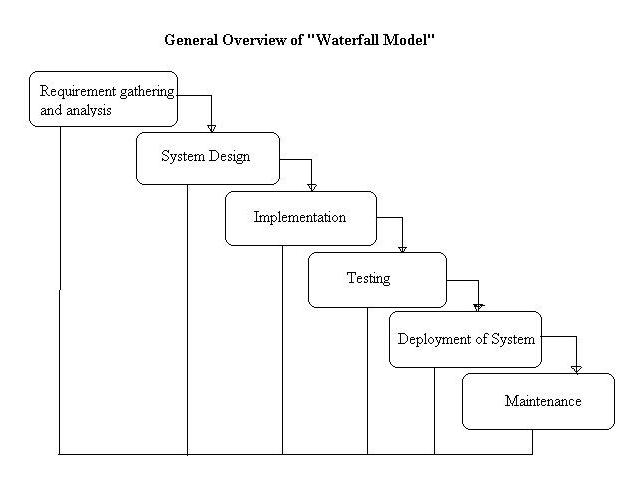
\includegraphics[width=1.0\textwidth]{Waterfall-model.jpg}
    \caption{An example of Waterfall development\cite{prototype}}
    \label{fig:waterfall-dev}
\end{figure}\\
\textbf{Advantages}:
\begin{itemize}
\item Clear project objectives.
\item Easy to understand and use.
\item Lack of alteration of requirements.
\item Progress of system is measurable.
\item Strict sign-off requirements. 
\end{itemize}
\textbf{Disadvantages}:
\begin{itemize}
\item Time consuming.
\item Once an application is in the testing stage, it is very difficult to go back and change something that was not well-thought out in the concept stage. 
\item Little room for iteration. 
\item Difficulty responding to changes.
\end{itemize}

\subsection{Prototyping Model}
This model involves creating a prototype which is not based on strict planning, but is an early approximation of the final product or software system. This prototype acts as a sample and is tested to help the developer learn and create a better final product. This model would be used when it is very difficult to obtain strict requirements. The prototype is redeveloped based on the feedback from the user so it is constantly gettin tested\cite{prototype}.
\begin{figure}[!htbp]
  \centering
    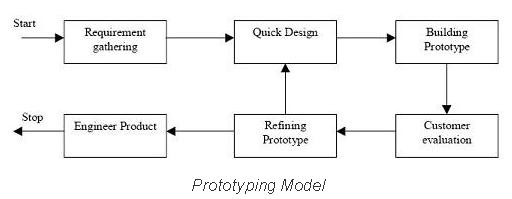
\includegraphics[width=1.0\textwidth]{Prototype-model.jpg}
    \caption{An example of Prototype development\cite{prototype}}
    \label{fig:prototype-dev}
\end{figure}\\
\textbf{Advantages}:
\begin{itemize}
\item Users are actively involved in the development
\item Since in this methodology a working model of the system is provided, the users get a better understanding of the system being developed.
\item Errors can be detected much earlier.
\item Quicker user feedback is available leading to better solutions.
\item Missing functionality can be identified easily
\item Confusing or difficult functions can be identified
\item Requirements validation, Quick implementation of, incomplete, but
functional, application. 
\end{itemize}
\textbf{Disadvantages}:
\begin{itemize}
\item Requirements may change drastically and frequently.
\item It can be time consuming if users continuously tweak demo after prototype. 
\item Since the demo is not really a complete working model, it can't find all the problems that will be in a full working version.
\item Incomplete or inadequate problem analysis. 
\item Approval process and requirement is not strict.
\end{itemize}

\subsection{Spiral Life Cycle Model}
The Spiral Life Cycle Model is a type of iterative software development model which is generally implemented in high risk projects. his method combines the features of both, waterfall model and prototype model. All the activities in the form of a spiral.
Each loop in a spiral represents a development phase with each loop has four sections or quadrants :
\begin{enumerate}
\item To determine the objectives, alternatives and constraints. 
\item Risk analysis and evaluation of alternatives. 
\item Execution of that phase of development. 
\item Planning the next phase. 
\end{enumerate}
Subsequent loops of spiral model involve similar phases. Analysis and engineering efforts are applied in this model. Large, expensive or complicated projects use this type of life cycle because if at any time the project is deemed too risky or uneconomical it can be aborted\cite{spiral}.
\begin{figure}[!htbp]
  \centering
    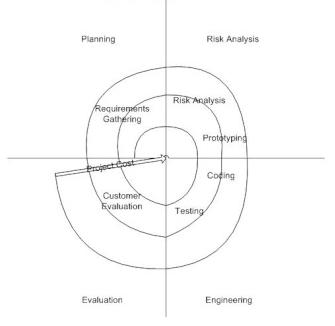
\includegraphics[width=1.0\textwidth]{Spiral-model.jpg}
    \caption{An example of Spiral development\cite{spiral}}
    \label{fig:spiral-dev}
\end{figure}\\
\textbf{Advantages}:
\begin{itemize}
\item Extremely flexible. 
\item Risk management is built in. 
\item Project monitoring is very easy and effective. Each phase, as well as each loop, requires a review.
\item Changes can be introduced later in the life cycle. 
\end{itemize}
\textbf{Disadvantages}:
\begin{itemize}
\item Highly expensive.
\item Complicated approach. 
\item Rules and protocols must be followed strictly.
\item Amount of documentation required in intermediate stages makes management of project very complex.
\end{itemize}

\subsection{Agile Model}
Agile development is a model that delivers a working application free of all known bugs at the end of each development iteration. The resulting application is then sent to the client for testing and feedback. This method emphasises interaction between developers and clients, and working software rather than progress reports. This model is generally used for time critical projects\cite{agile}.
\begin{figure}[!htbp]
  \centering
    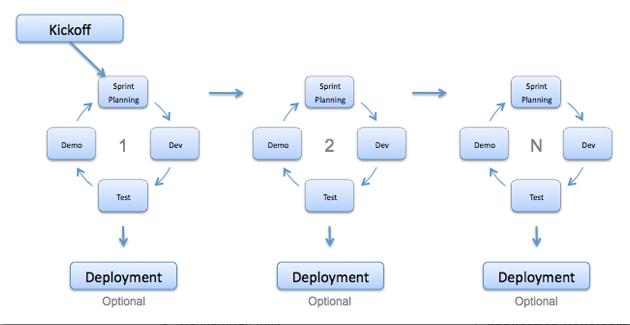
\includegraphics[width=1.0\textwidth]{agile-dev.jpg}
    \caption{An example of Agile development\cite{agile}}
    \label{fig:agile-dev}
\end{figure}\\
\textbf{Advantages}:
\begin{itemize}
\item Working software is delivered frequently.
\item Very high levels of customer satisfaction. 
\item Working software is the main measure of progress.
\item Flexibility in requirements changes.
\item Simplicity.
\item Adaptable to changing circumstances.
\end{itemize}
\textbf{Disadvantages}:
\begin{itemize}
\item Requires very experienced developers who understand business and administration as well as software development as it is difficult to assess the effort required at the beginning of the software cycle.
\item Lack of emphasis on designing and documentation.
\end{itemize}

\subsection{Software Development Model Chosen and Why}
After much research the Agile development model was chosen as the most suitable for this project, and there were many numerous for this choice. First and foremost, the project had a strict deadline which suits this development model. Another reason for choosing agile was its flexibility. Due to lack of experience in software development it was assumed that the requirements would change quite often. Through this model the project could easily adapt and promote rapid progression through frequent development iterations. 
Overall the agile approach suited best as it allows for creation of a highly functional project within a strict time frame.  

\section{Storing Data}
The project required storage of data to work correctly. A users details must be stored along with the information for each station and song. During the design phase decisions had to be made on what method would be best for his storage of data. The research done on existing applications came in very useful for this decision. \\

For a web application like this a relational database is the best choice. A relational database is a collection of data items organized as a set of formally-described tables from which data can be accessed or reassembled in many different ways without having to reorganize the database tables\cite{RDSM}. The most popular relational databases are Oracle, MySQL, Microsoft SQL Server and PostgreSQl. 

\subsection{Oracle}
Oracle is the best database for mission critical commercial applications. It ensure high level security by performing each transaction in isolation form others and ensures high level availability by providing solutions for fixing problems rapidly and minimize both planned and unplanned downtime. 

The downside to Oracle database systems is that they are high in cost and not open source so it did not make sense to use it for this project\cite{oracle}.

\subsection{MySQL}
MySQL is used in almost all open source web projects that require a database in the back-end. MySQl is part of the powerful LAMP stack along with Linux, Apache, and PHP. There is ample documentation online which would make using this relational database much easier\cite{MySQL}. 

\subsection{PostgreSQl} 
PotgreSQl is a open source object-relational database system. It runs on most *nix flavours, Windows and Mac OS\cite{PostgreSQL}. 

\subsection{Microsoft SQL Server}
Microsoft SQL Server again is very popular with businesses like Oracle is but due to the fact that it is not open source it was not chosen as the relational database for this project\cite{microsoftSQl}.

\subsection{Relational Database Chosen and Why}
MySQL was chosen as the relational database for this project for many reasons. Firstly it is by far the most popular relational database used today. The other main reason was the high levels of documentation online. Due to the tight time constraints set on this project it was felt that this would be the smart choice.

\section{Website Architecture}
Website architecture is an approach to the design and planning of website which, like architecture itself, involves technical, aesthetic and functional criteria\cite{web_arch}. This means planning out what web pages will exist and how they link together. \\

\subsection{Bad Website Architecture}
Poorly designed websites occur due to lack of planning. Usually website with a bad structure have been hacked together and cross linked so much it is near impossible to navigate efficiently. A key design flaw for these websites is that you must navigate through many pages in order to get to your destination. Good practice in regards to web architecture would be that no web page is more than three clicks away form the homepage.
\begin{figure}[!htbp]
  \centering
    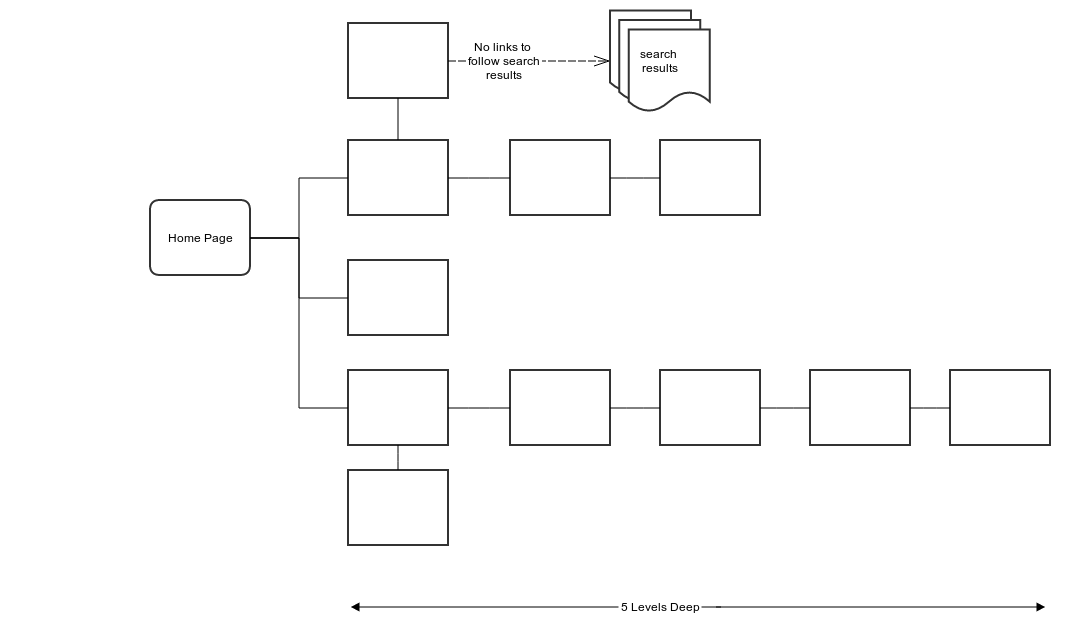
\includegraphics[width=1.0\textwidth]{bad_web_arch.png}
    \caption{An example of bad web architecture}
    \label{fig:bad_web_arch}
\end{figure}\\

\subsection{Good Website Architecture}
In good website architecture the main things to consider would be;
\begin{itemize}
\item Minimal click-depth.
\item How each page is linked internally.
\item Avoiding the big issues at the start eg. duplicate urls, minimal code for fast pages 
\end{itemize}
As stated previously under bad website architecture good practice states that no pages should be more than 3 levels deep. Figure~\ref{fig:good_web_arch} shows a good example of how a website should be laid out where any page can be accessed in a maximum of three clicks from the homepage.
\begin{figure}[!htbp]
  \centering
    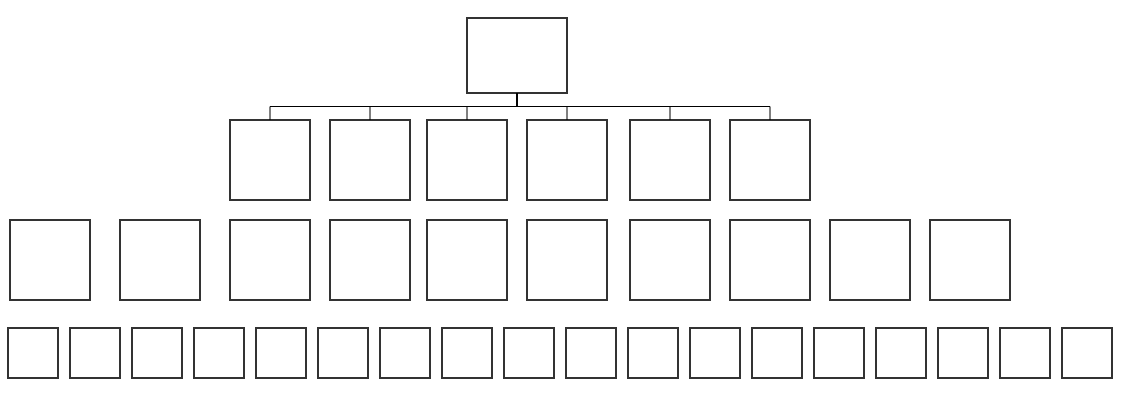
\includegraphics[width=1.0\textwidth]{good_web_arch.png}
    \caption{An example of good web architecture}
    \label{fig:good_web_arch}
\end{figure}

\section{Navigation}
Navigation in web design is very important and plays a major role in a website's usability and ensuring a positive user experience.   
The navigation menu on a website is like sign post on the street or a map in a building. You cannot reach your destination without first knowing where you are. \\
While designing a good navigation system the following sections should be taken into account:
\begin{itemize}
\item Information Architecture.
\item Use of User-Enabled Technologies.
\item Using Simple Terms.
\item Standardisation.
\item Indication of Current Location.
\item Use of Web Conventions.
\end{itemize}

\subsection{Information Architecture}
The first step of navigation planning is information architecture\cite{IA_101}. This consists of planning what features the website offers, what features and most important and what features can be placed in lower levels of the the information hierarchy. 
An index page hierarchy was chosen for this project. This consists of a main page which serves as a launch pad for the other pages. 

\subsection{Use of User-Enabled Technologies}
The use of Flash, JavaScript, JQuery or anything else that may inhibit access to the website through its navigation menu should be avoided but if it cannot be the user should be able to degrade gracefully\cite{fallback_css_js}.

\subsection{Using Simple Terms}
Simple, obvious terms that are easy to figure out should be used for the navigation menu. Any link that takes users more than a second or two to figure are unsuitable for use. If a user needs to click on a link to figure out what the link leads to then this will contribute to a bad user experience for your visitors. 

\subsection{Indication of Current Location}
To insure a positive user experience the user should always know where they are in the site at all times. This can be done either changing the links background of the colour of the page name to make it different from the other elements in the navigation menu.

\subsection{Use of Web Conventions}
It is all about easy-to-use and intuitive website navigation. Web conventions make it a lot easier for designers to work around their designs. Most users would click on the website logo to get back to the homepage, so design your logo to do that.

If you don’t, you are making them spend time to learn something new or in some cases inconvenience them by not providing what they expect to be commonly accepted navigational norms.

When designing the navigation menu their are certain web conventions\cite{web_design_conventions} that should be taken into account. Using these conventions will help make the site easy-to-use and improve the user experience. An example of a web convention would be clicking the website logo that would be in the top left corner of the site would return the user to the homepage. By not using these conventions you will inconvenience the user by not providing what they expect to be commonly accepted navigation practices.

\section{Use Cases}
During the development of this project many use cases were defined. A use case defines the interactions between an external actor who is the user and the system to attain particular goals. They are used to help plan a systems features in advance and how the user will interact with it to achieve its goals.
Due to restrictions in space for this report I have only included four of the use cases created.\\ 
\textbf{Use Case:} Connect to a live station\\
\textbf{Actor:} Any user\\
\textbf{Steps:}
\begin{enumerate}
\item Go to homepage.
\item Browse displayed stations.
\item Click 'view station' button corresponding to desired station.
\end{enumerate}
\begin{figure}[!htbp]
  \centering
    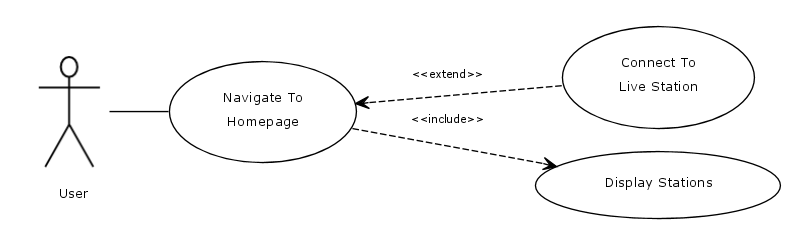
\includegraphics[width=1.0\textwidth]{usecase1.png}
    \caption{Use case diagram for connect to a live station}
\end{figure}
\textbf{Use Case:} Create station\\
\textbf{Actor:} Registered user\\
\textbf{Steps:} 
\begin{enumerate}
\item Go to homepage.
\item Login.
\item Select 'Create Station' in navigation menu.
\item Select desired songs from personal library.
\item Fill in Station Name field with a string value.
\item Fill in the Description field with a string value.
\item Select one of the multiple genre options.
\item Select one of the five station types.
\item Click 'Create Station' button.
\item Click 'Yes' button in confirmation pop-up.
\end{enumerate}
\begin{figure}[!htbp]
  \centering
    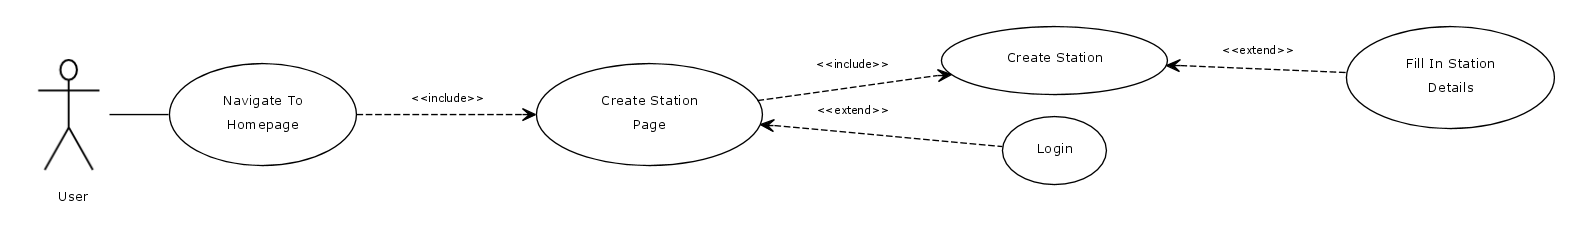
\includegraphics[width=1.0\textwidth]{usecase2.png}
    \caption{Use case diagram for create station}
\end{figure}
\textbf{Use Case:} Edit station\\
\textbf{Actor:} Registered user\\
\textbf{Steps:} 
\begin{enumerate}
\item Go to homepage.
\item Login.
\item Browse your displayed stations.
\item Click 'edit station' button corresponding to desired station.
\item Edit selected songs.
\item Edit Station Name field with a string value.
\item Edit the Description field with a string value.
\item Select one of the multiple genre options.
\item Select one of the five station types.
\item Click 'Save Changes' button.
\item Click 'Yes' button in confirmation pop-up.
\end{enumerate}
\begin{figure}[!htbp]
  \centering
    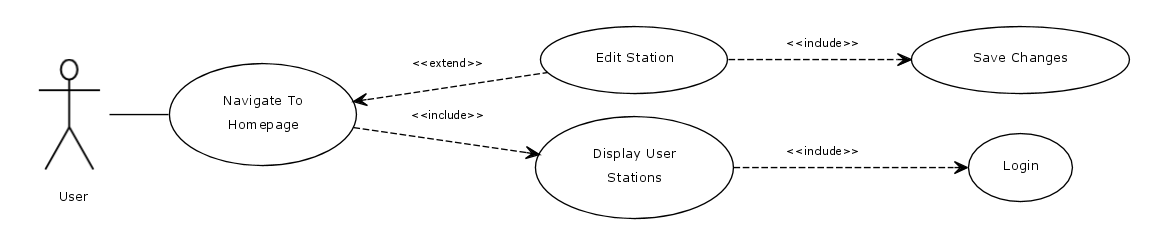
\includegraphics[width=1.0\textwidth]{usecase3.png}
    \caption{Use case diagram for edit station}
\end{figure}
\textbf{Use Case:} upvote song in station\\
\textbf{Actor:} Any user\\
\textbf{Steps:} 
\begin{enumerate}
\item Connect to live station.
\item Browse song list available.
\item Click 'Vote Up' button.
\end{enumerate}
\begin{figure}[!htbp]
  \centering
    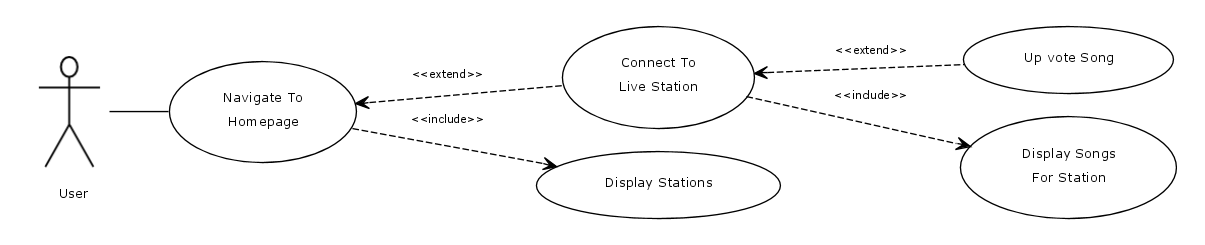
\includegraphics[width=1.0\textwidth]{usecase4.png}
    \caption{Use case diagram for upvote song in station }
\end{figure}

\section{Page Design}
During the research phase many available interfaces were tested. The advantages and disadvantages were taken into account during this phase of designing each page of the web application.

\subsection{Home Page}
As an index page hierarchy was chosen for this project the home page would be a launch pad most the main features. To include the differing features available to logged in users and non signed in users two separate home pages were designed. As shown in Figure~\ref{homepage-anon} the homepage for non signed in users displays all the current live stations being broadcast by other users. It was decided that displaying all these stations in a simple table that is sortable by each header Station Name, User Name, Genre, Description, and Station Type was the most efficient way of displaying them. Also it follows well known web conventions associated with displaying large amount of information. For each station displayed in the table there is a button 'view station' which when clicked will allow the user to connect to the station. \\
\begin{figure}[H]
  \centering
    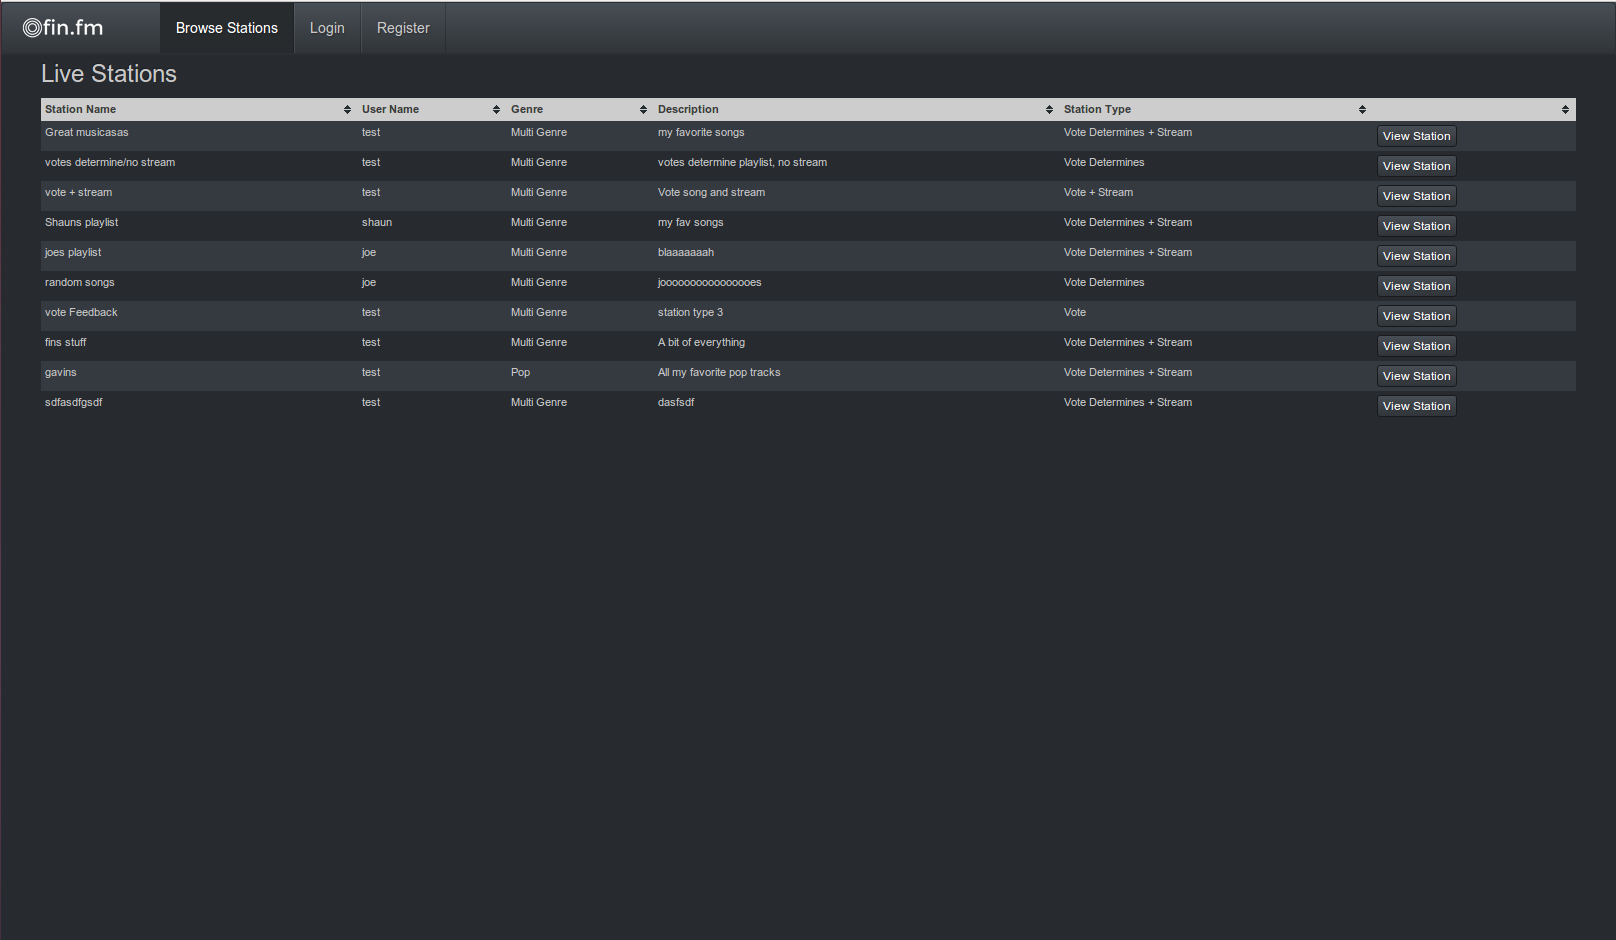
\includegraphics[width=1.0\textwidth]{screenshots/homepage-anon.png}
    \caption{The homepage for non signed in users}
    \label{homepage-anon}
\end{figure}
The navigation menu only provides two options for the user. These links cause either login form or a register form to appear in a iframe seen in figures~\ref{login} and ~\ref{register} respectively when either of these forms is completed it will bring the user to the homepage for logged in user seen in figure~\ref{homepage}.\\
\begin{figure}[H]
  \centering
    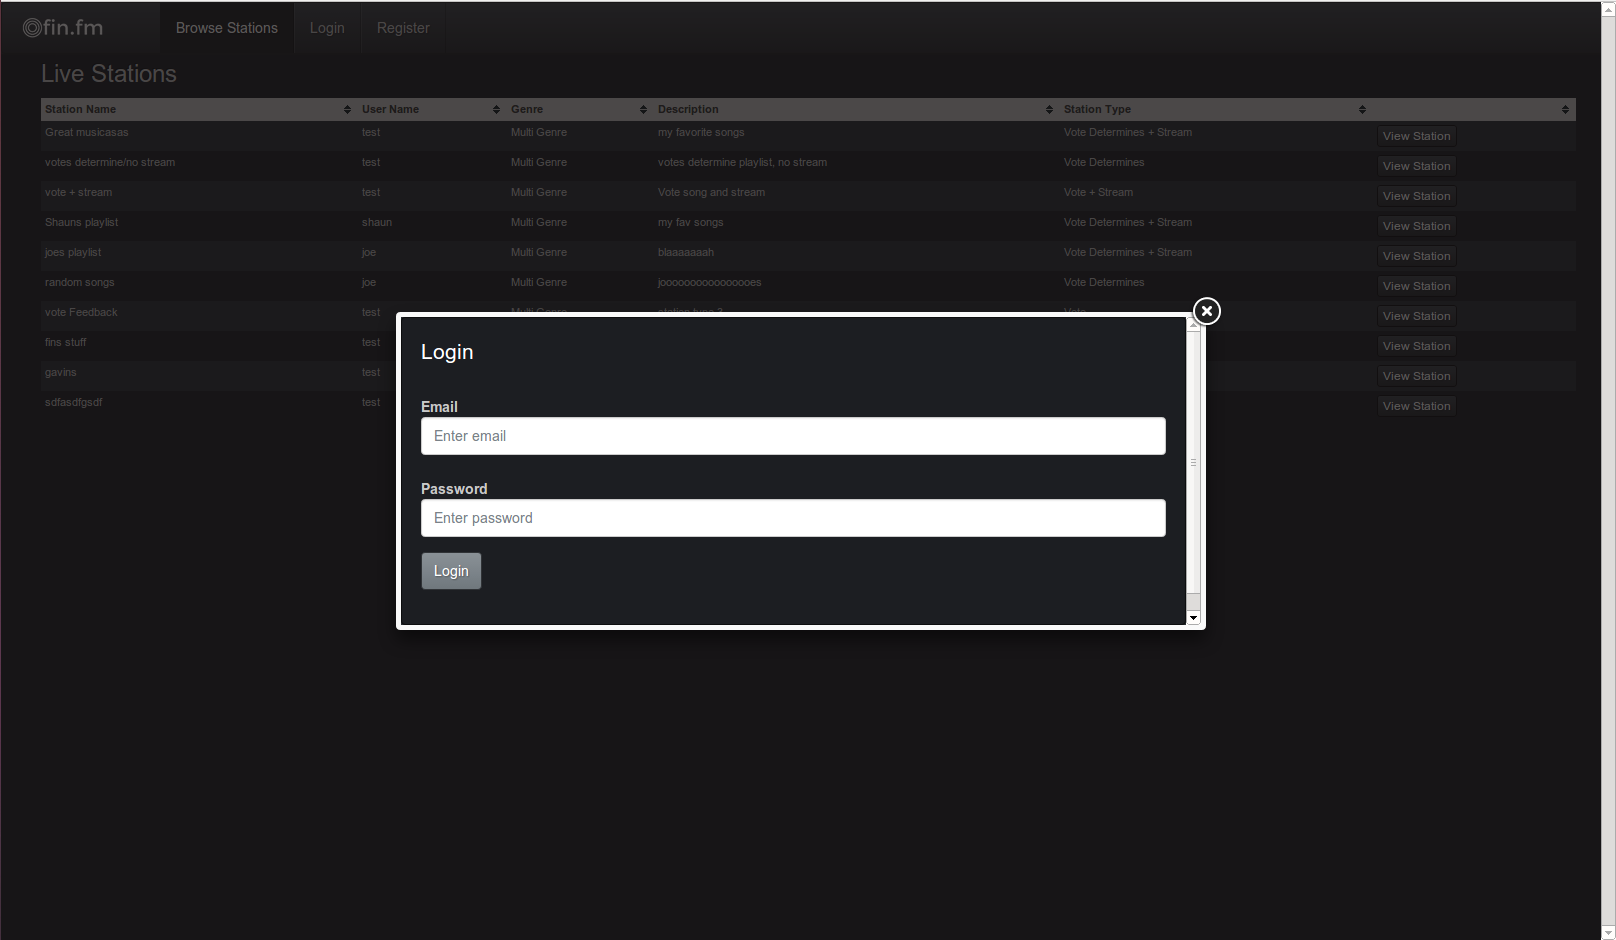
\includegraphics[width=1.0\textwidth]{screenshots/login.png}
    \caption{The login iframe}
    \label{login}
\end{figure}
\begin{figure}[H]
  \centering
    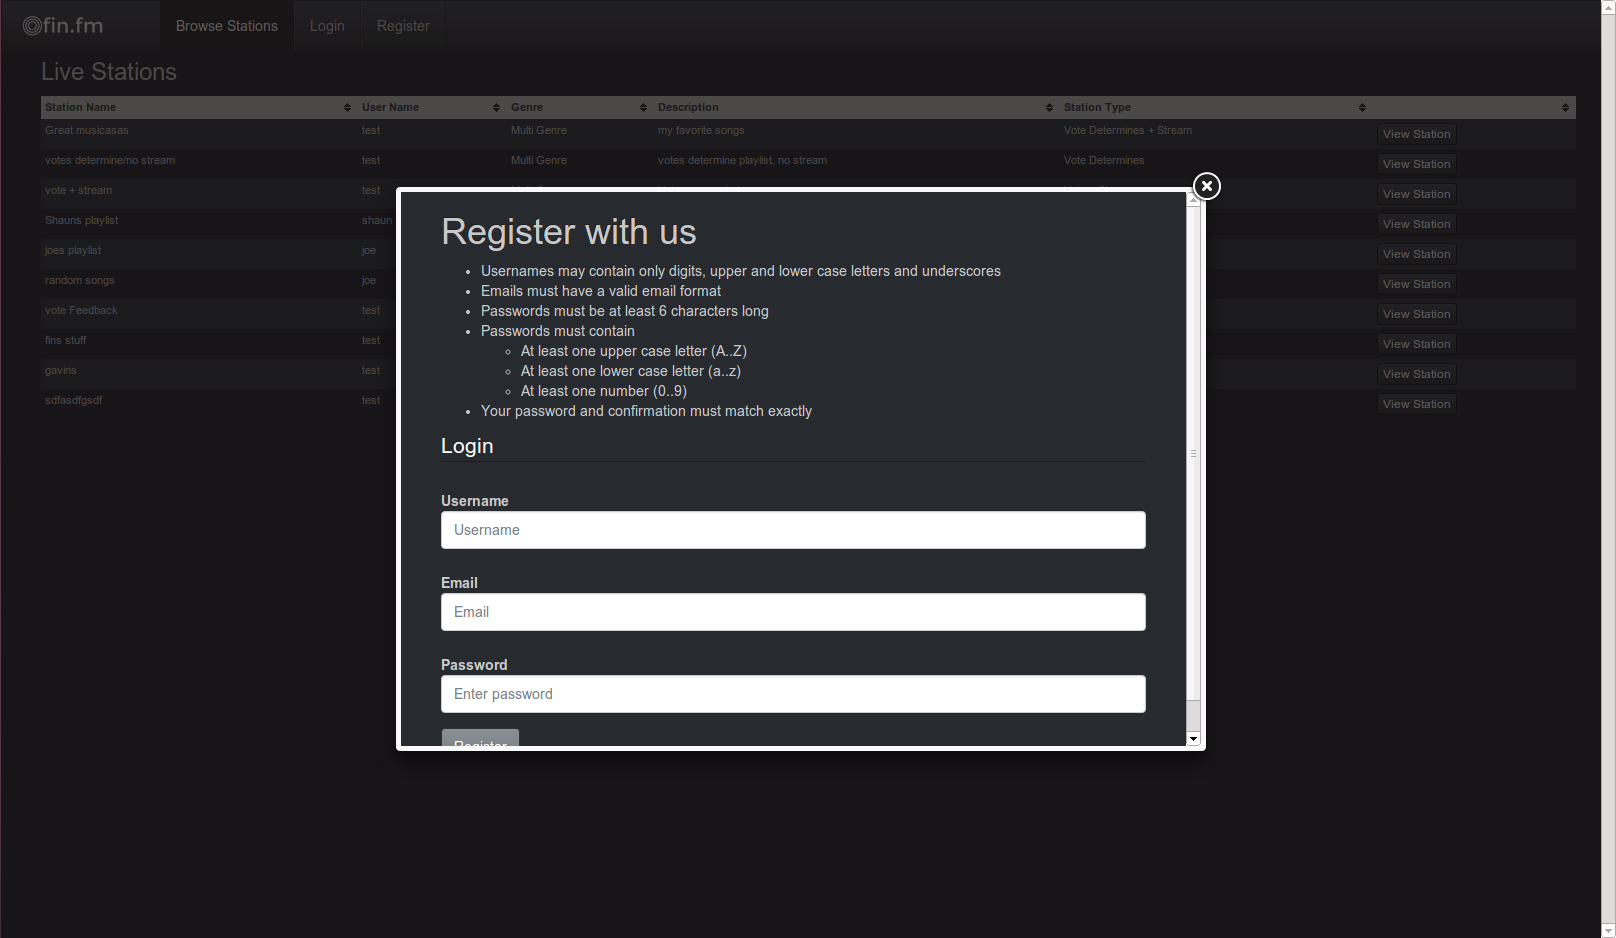
\includegraphics[width=1.0\textwidth]{screenshots/register.png}
    \caption{The register iframe}
    \label{register}
\end{figure}
\begin{figure}[H]
  \centering
    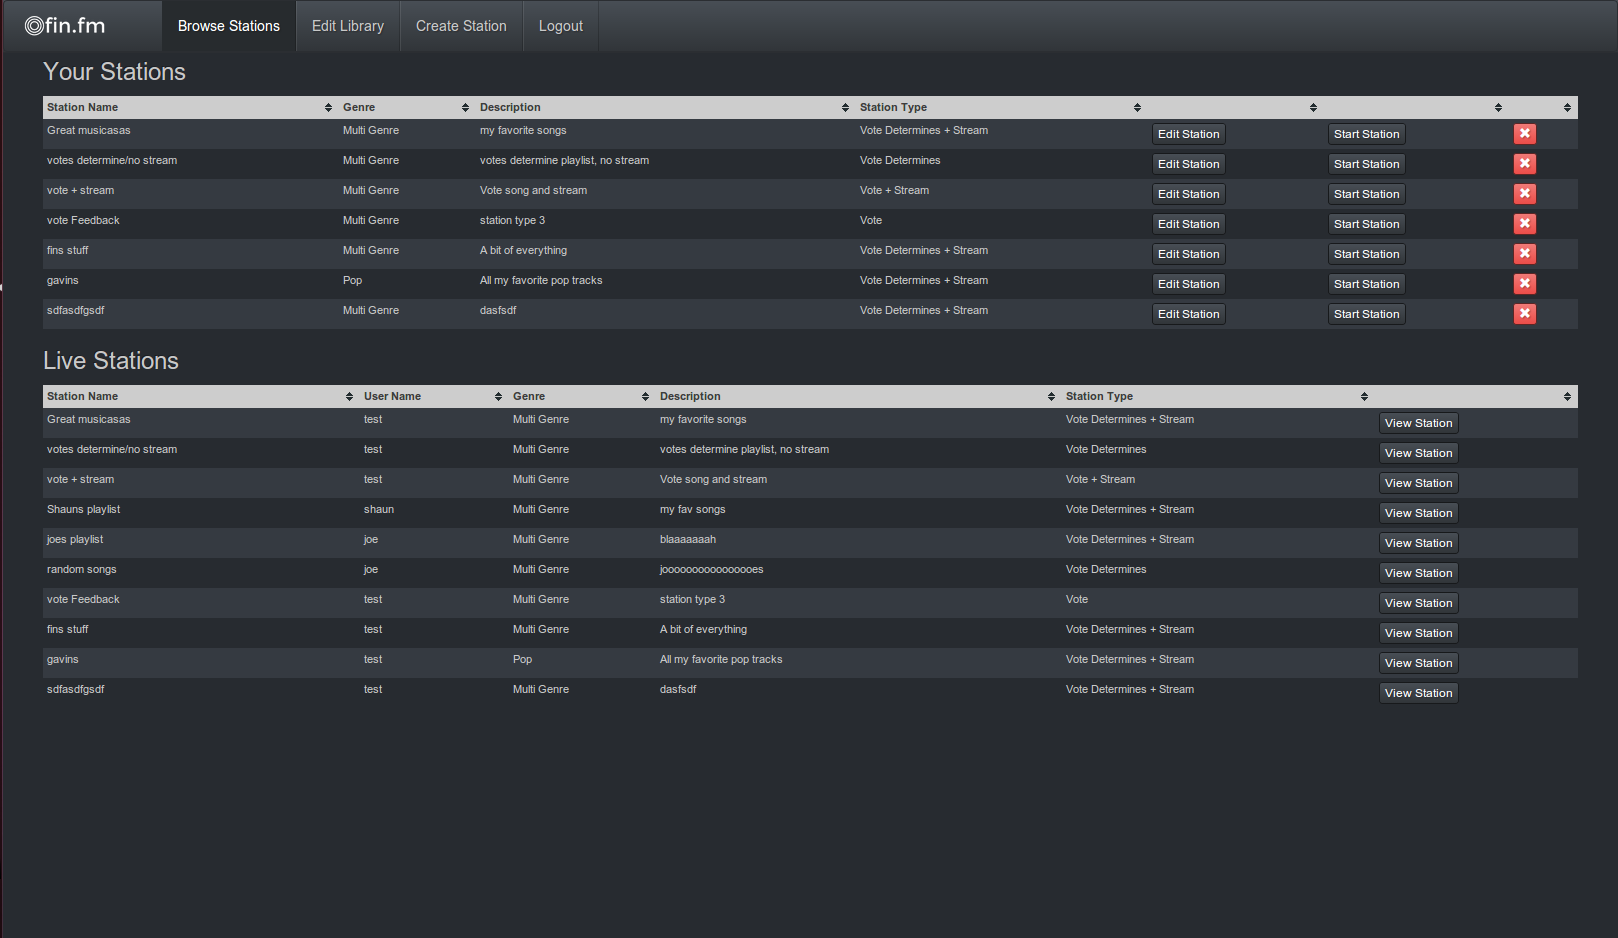
\includegraphics[width=1.0\textwidth]{screenshots/homepage.png}
    \caption{The homepage for logged in users}
    \label{homepage}
\end{figure}
The homepage for logged in users seen in figure~\ref{homepage} is quite different from the homepage for non signed in users but also has some similarities. For this homepage the current live stations being broadcast by other users are still displayed in the same way but there is also a separate table table which displays the stations owned by the user. Instead of the the 'view station' button that is in the table displaying the current live stations there are two separate buttons. One which send users to a page where they can edit that particular station with the name of 'Edit Station' and the other a red button with and 'X' which allows users delete a station. The choice to use a red button with an 'X' follows the well known web convention which users can assume means delete. 
When the delete button is clicked users are promtped with a confirmation box shown in figure~\ref{delete-confirm} to make sure they mean to delete their station  \\
\begin{figure}[H]
  \centering
    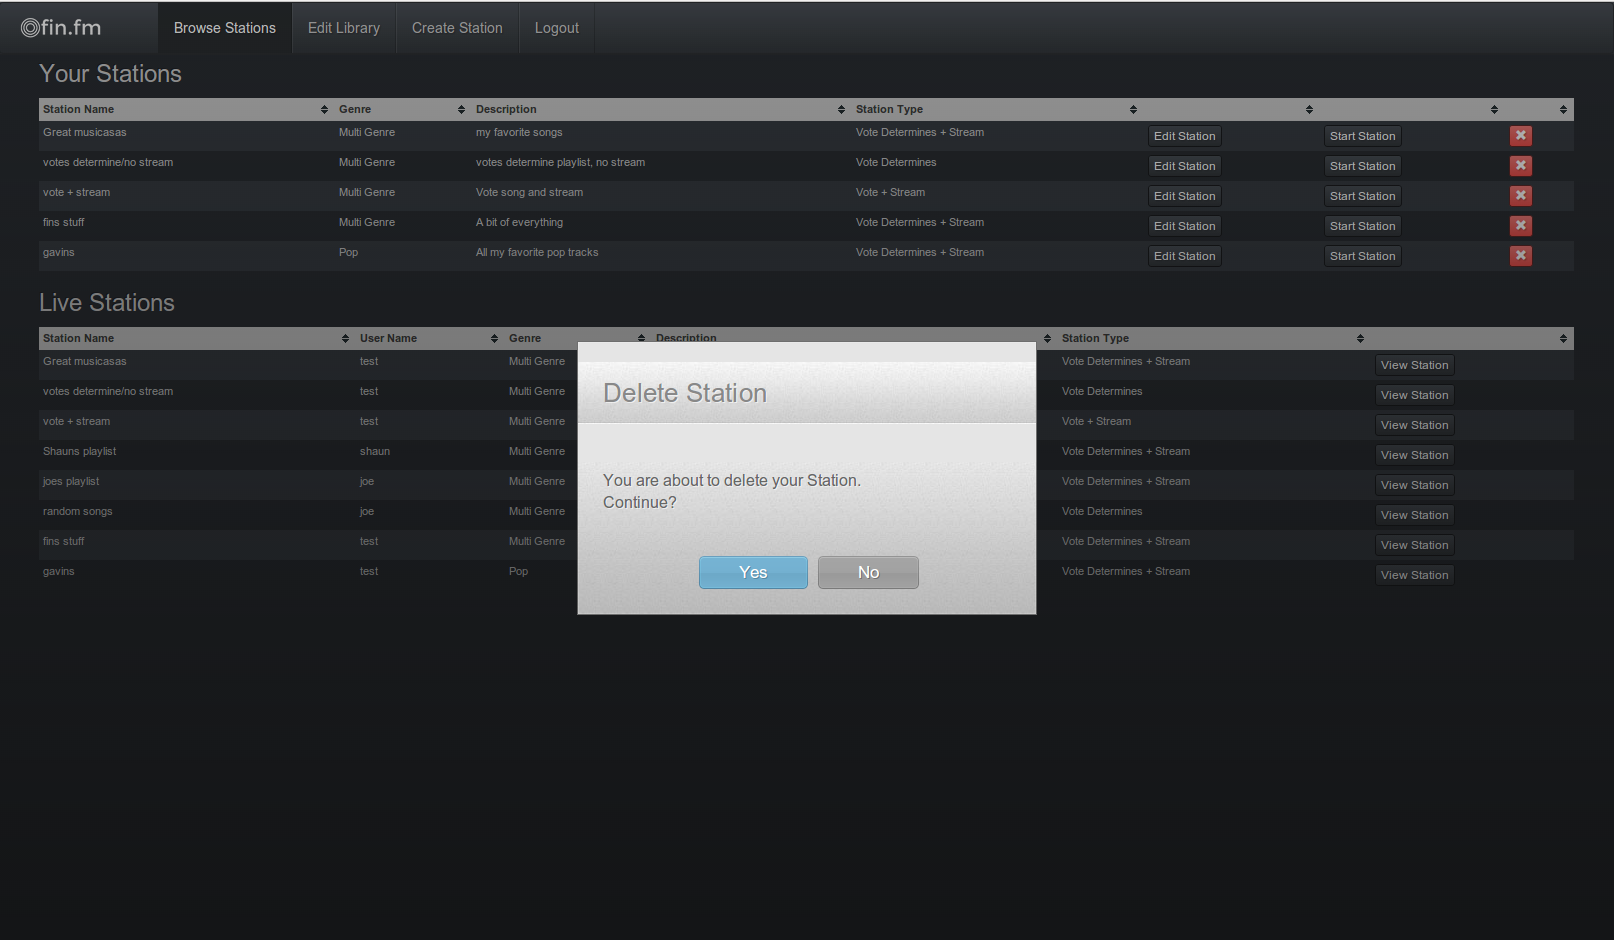
\includegraphics[width=1.0\textwidth]{screenshots/delete-station-confirm.png}
    \caption{Delete station confirmation}
    \label{delete-confirm}
\end{figure}
The navigation menu is also different for logged in users. Instead of displaying Browse Stations, Login and Register it now displays links to  Browse Stations, Edit Library, Create Station and Logout. If a users clicks Logout they will be logged out and sent to the homepage for non signed in users.

\subsection{Create Station Page}
When a user selects to create a station they are sent to page containing a form as seen in figure~\ref{create station}. This page keeps a consistent style the same as the homepage. While creating the station users must firstly select what songs they want to use from their personal library. These songs are chosen from a table which displays all the songs from the users personal library with a checkbox for each. This table is consistent with the tables shown in the homepage.\\
Once the user has selected the desired songs from their personal library they then fill in the station information. This consists of Station Name, Description, Genre and Station Type. When this has all been completed the user then clicks the 'Create Station' button which prompts a confirmation box as seen in figure~\ref{create-confirm}. If the user decides to confirm the creation of the station they are brought to the respective live broadcast control page for that station.
\begin{figure}[H]
  \centering
    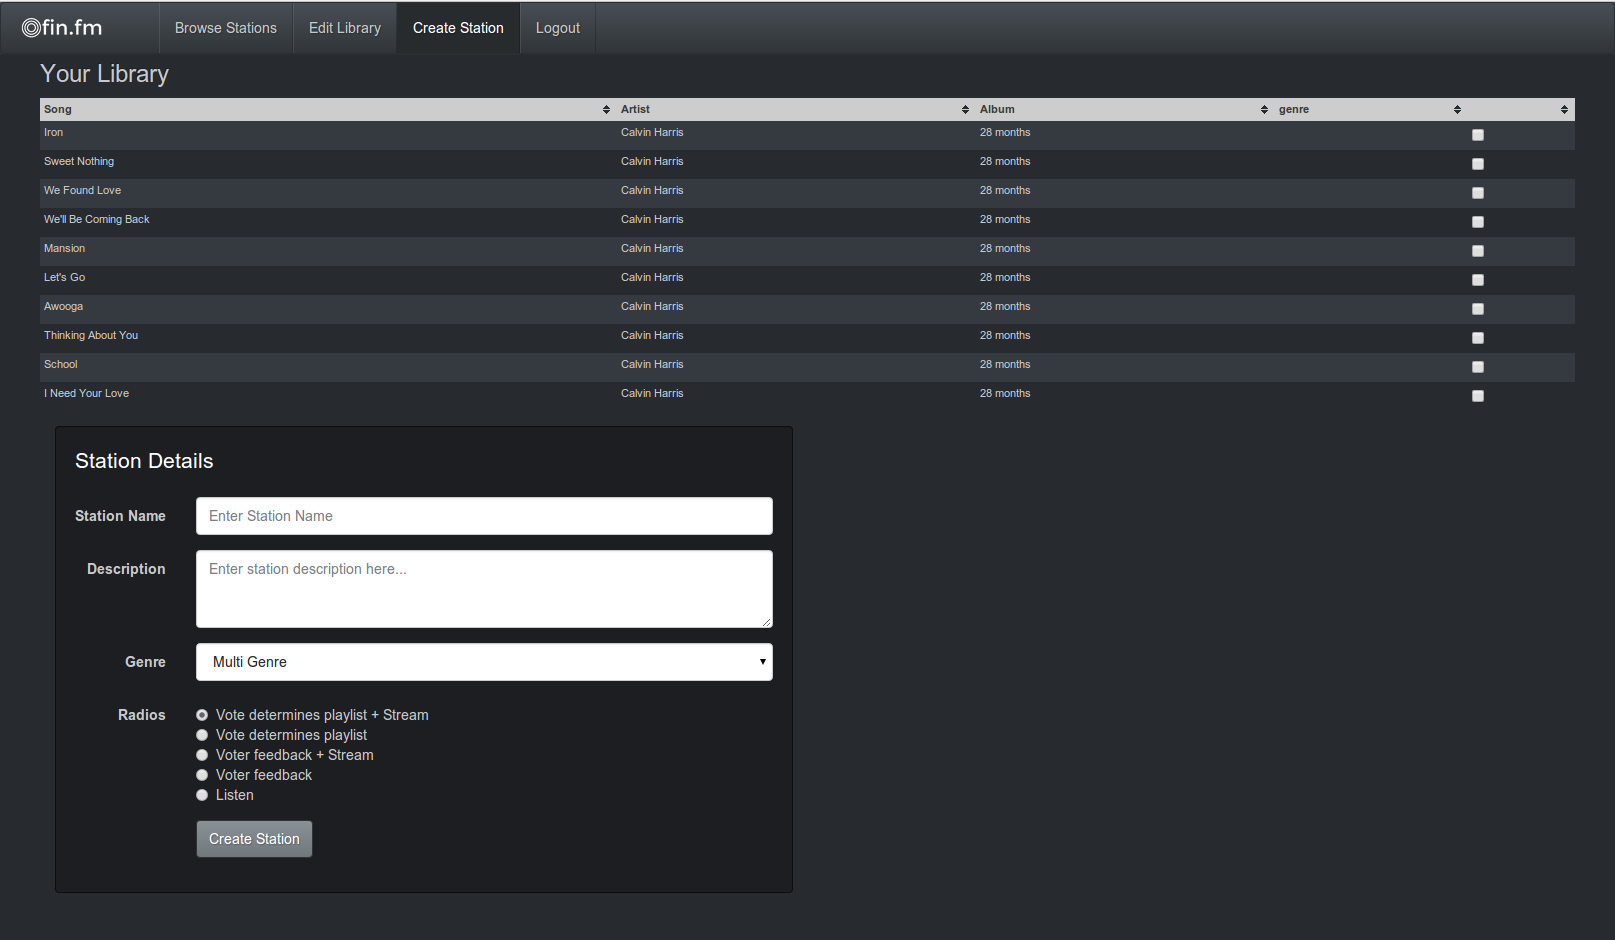
\includegraphics[width=1.0\textwidth]{screenshots/create-station.png}
    \caption{Create station page}
    \label{create station}
\end{figure}
\begin{figure}[H]
  \centering
    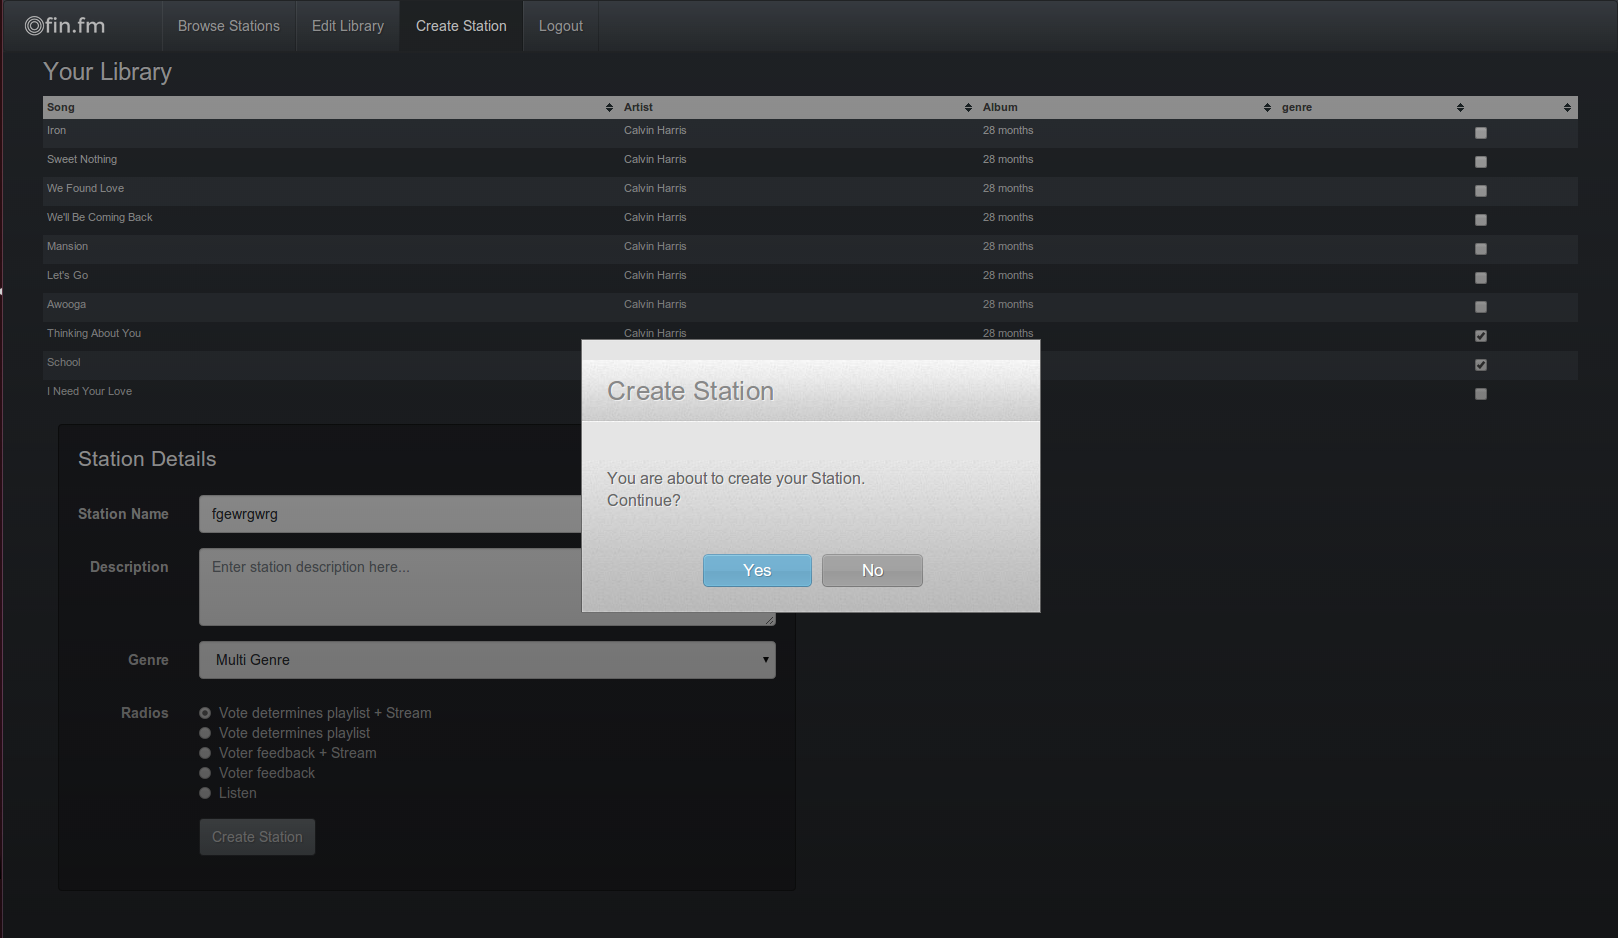
\includegraphics[width=1.0\textwidth]{screenshots/create-station-confirm.png}
    \caption{Confirm creation of station}
    \label{create-confirm}
\end{figure}
\subsection{Edit Station Page}
If a logged in user decides to click the 'edit station' button displayed for their personal stations on the homepage then they are sent to the edit stations page seen in figure~\ref{edit-station}. This page is almost a complete copy of the create stations page seen in figure~\ref{create station} but the songs already selected for this station are already checked along with the station information being filled in or selected for the corresponding to the stations current configuration. 
When a user has made their desired alterations they click the 'Save Changes' button which prompts a confirmation box as seen in figure~\ref{edit-station-confirm}.
\begin{figure}[H]
  \centering
    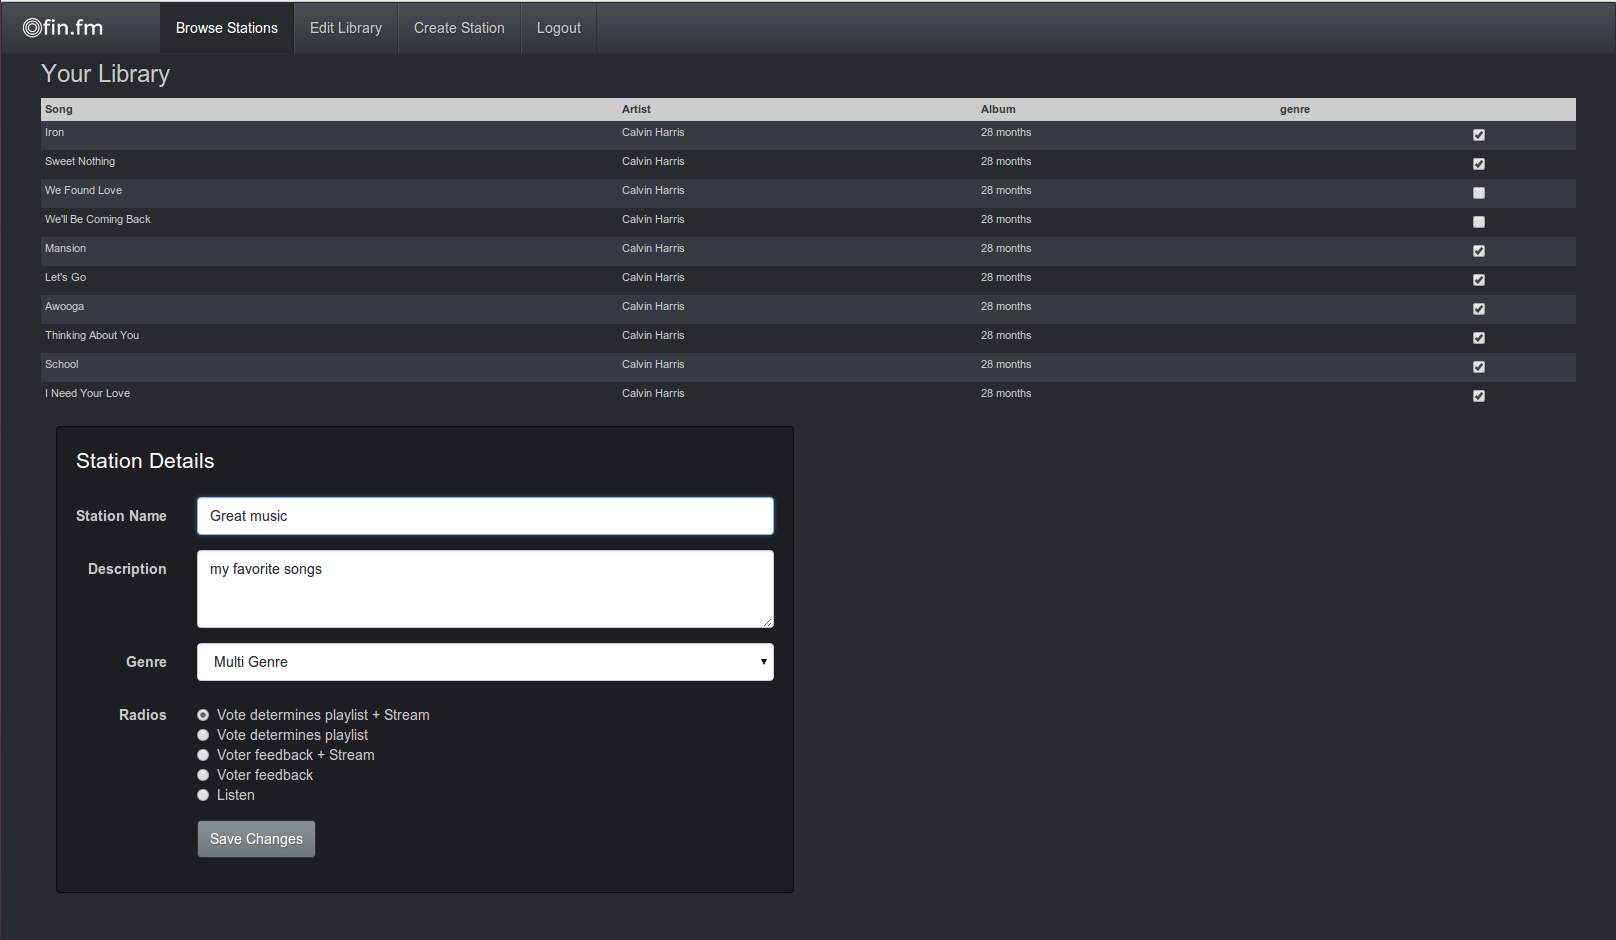
\includegraphics[width=1.0\textwidth]{screenshots/edit-station.png}
    \caption{Edit station page}
    \label{edit-station}
\end{figure}
\begin{figure}[H]
  \centering
    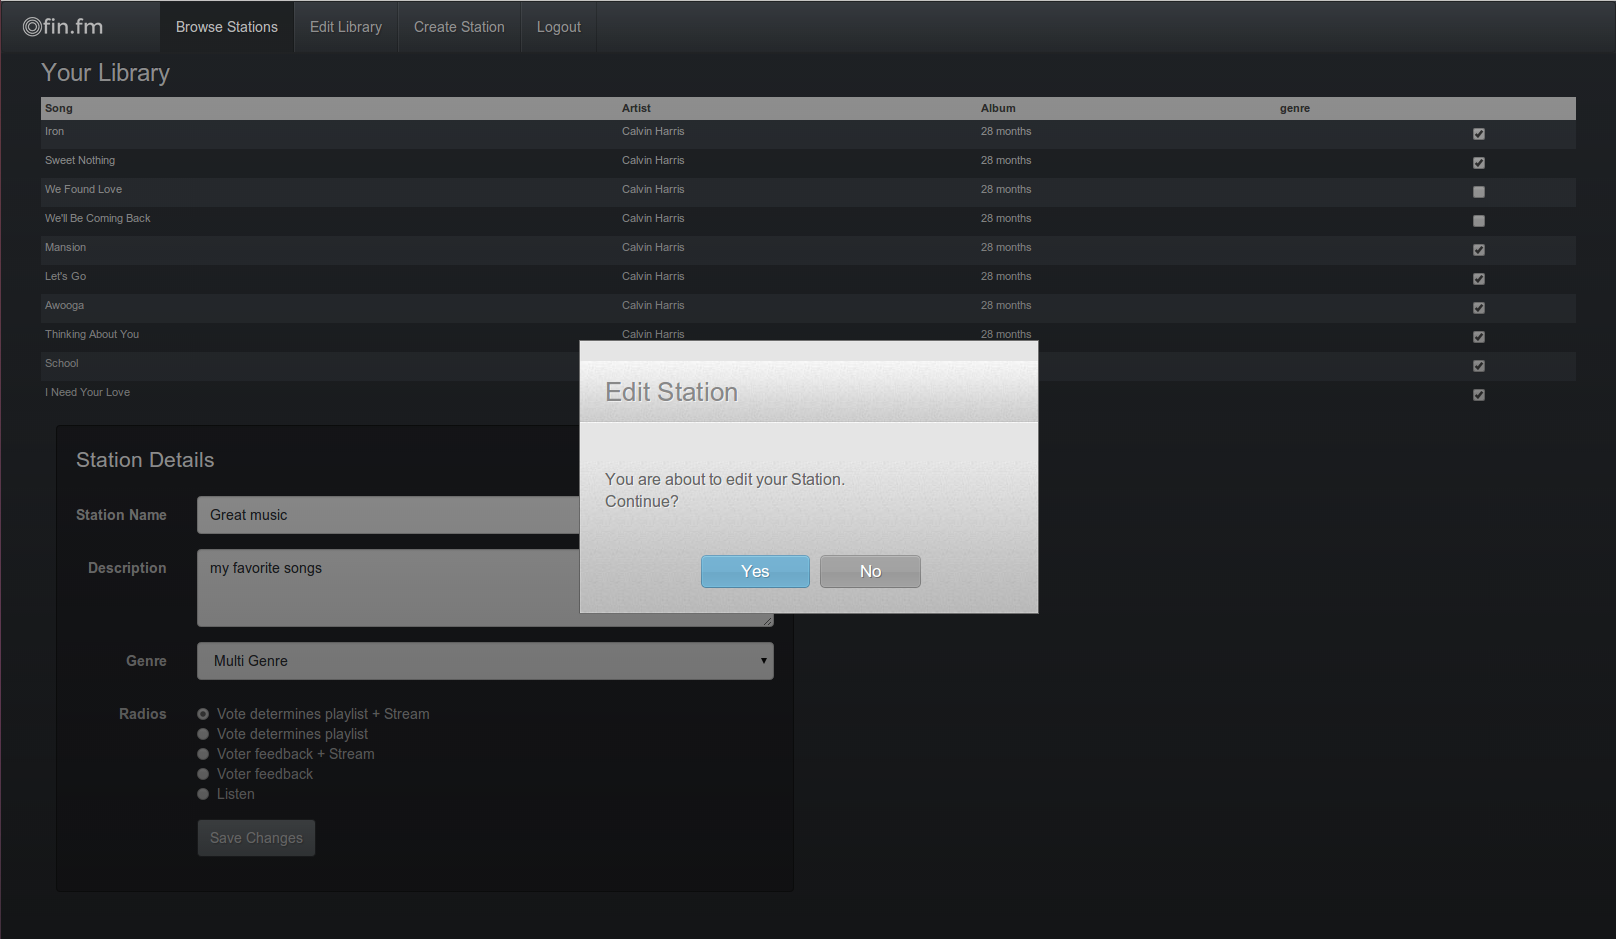
\includegraphics[width=1.0\textwidth]{screenshots/edit-station-confirm.png}
    \caption{Confirmation of station edit}
    \label{edit-station-confirm}
\end{figure}
\subsection{Edit Library Page}
A signed in user has the ability to create a personal library. With this library users can then create stations. Users can add or remove songs from this library through the edit library page. 
The contents of the users personal library are displayed in a table format at the beginning of the page. Each song has a corresponding check box which is checked and the 'Delete Checked Items' button is clicked will be removed from the personal library. This can be seen in figure~\ref{edit-library}. To ensure that users do not inadvertently delete songs a confirmation box as seen in figure~\ref{edit-library-confirm} is prompted when the 'Delete Checked Items' button is clicked.
\begin{figure}[H]
  \centering
    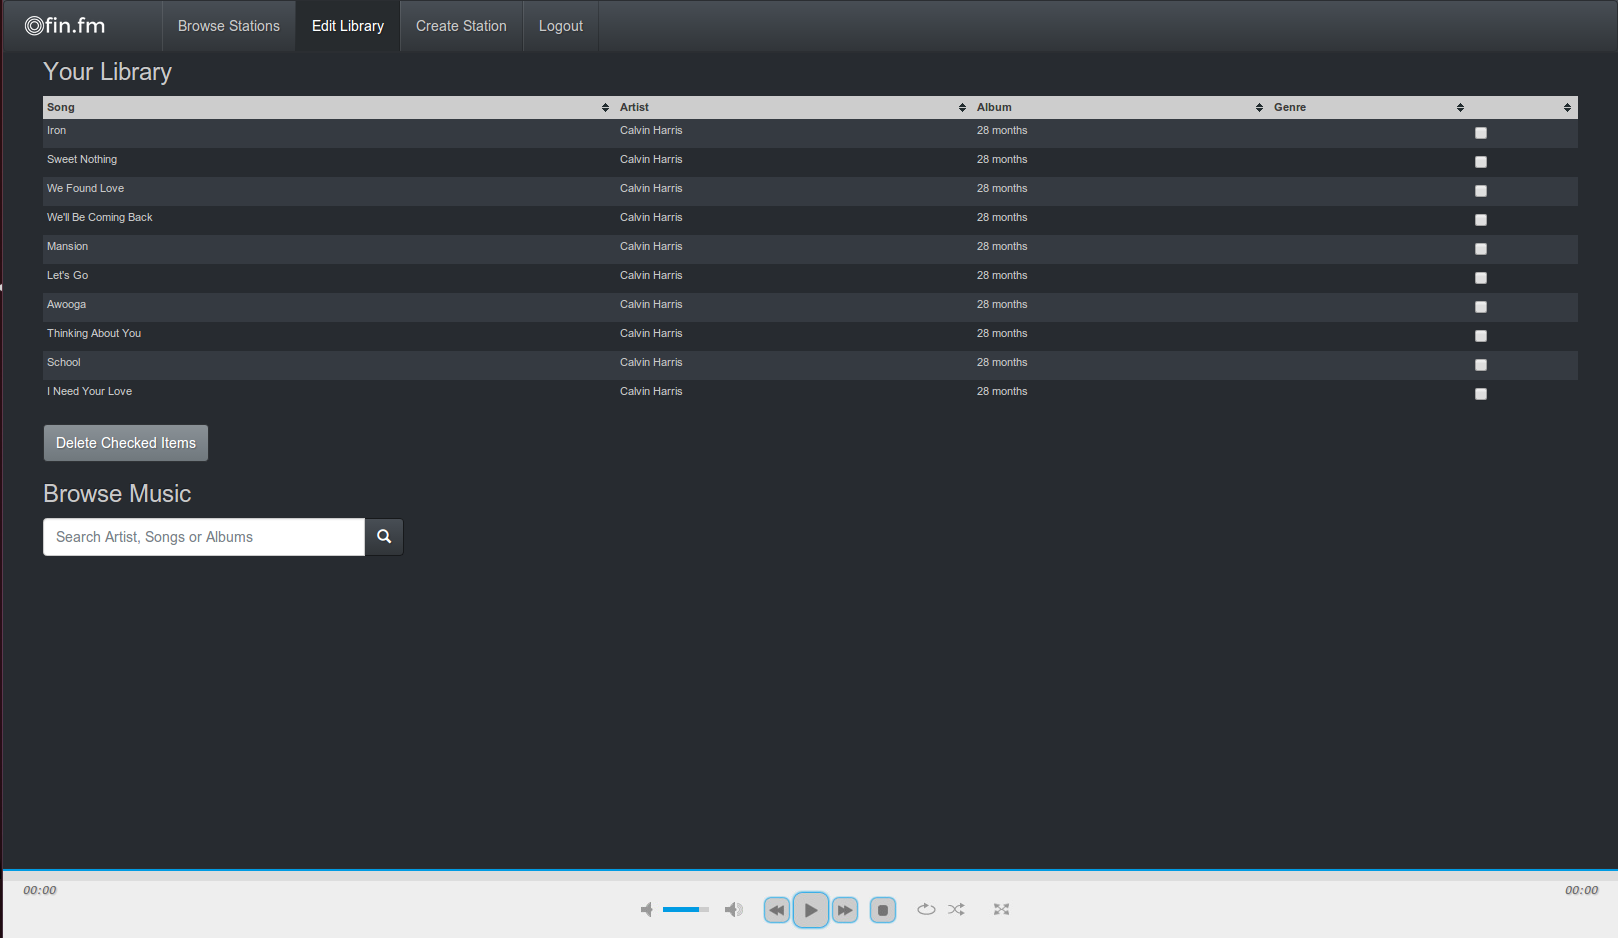
\includegraphics[width=1.0\textwidth]{screenshots/edit-library.png}
    \caption{Edit personal library page}
    \label{edit-library}
\end{figure}
\begin{figure}[H]
  \centering
    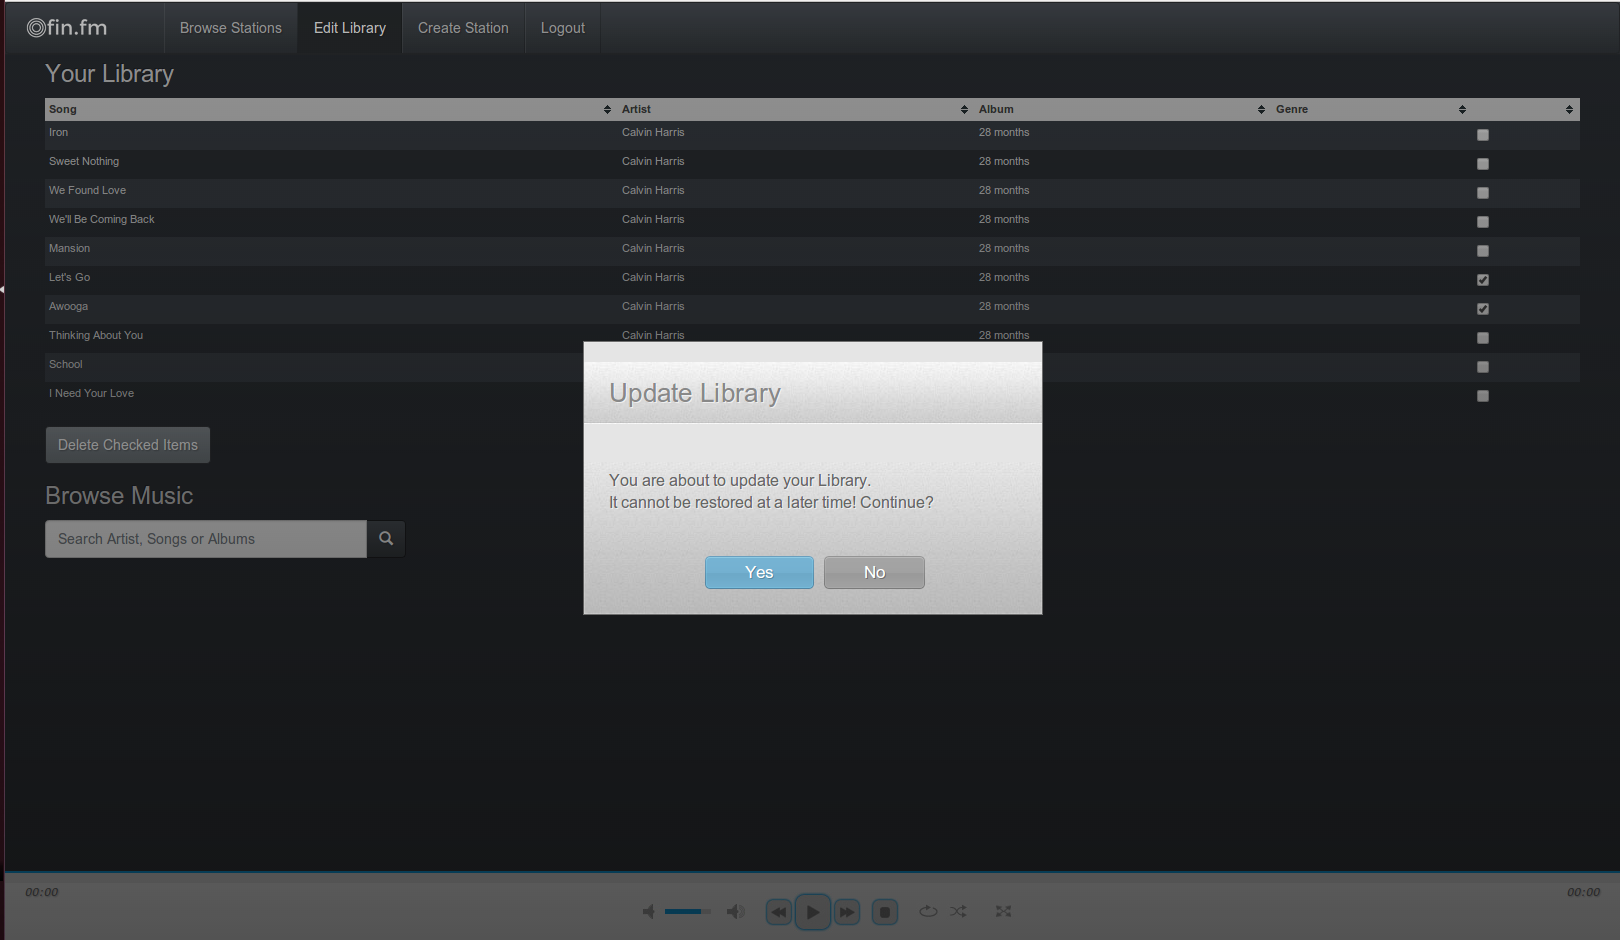
\includegraphics[width=1.0\textwidth]{screenshots/edit-library-confirm.png}
    \caption{Confirm edit of station}
    \label{edit-library-confirm}
\end{figure}
From this page users can also browse the entire user curated library consisting of every song uploaded by all other users. This library can be searched through the textfield which follows he web constant of having a magnifying glass as a button which is widely know to represent 'search'. When a query is entered it is search against song name, artist name, and genre and a resulting page as seen in figure~\ref{browse-library} will be generated.
The generated search results are displayed in a table format with two buttons corresponding to each item. The first button 'Add To Library' when clicked will add this particular song to the users personal library if it does not already exist. The second button 'Add To Playlist' adds the song corresponding to this button to the media player at the bottom of the page. This allows the user to listen to the song before deciding whether or not to add it to their personal library.   
\begin{figure}[H]
  \centering
    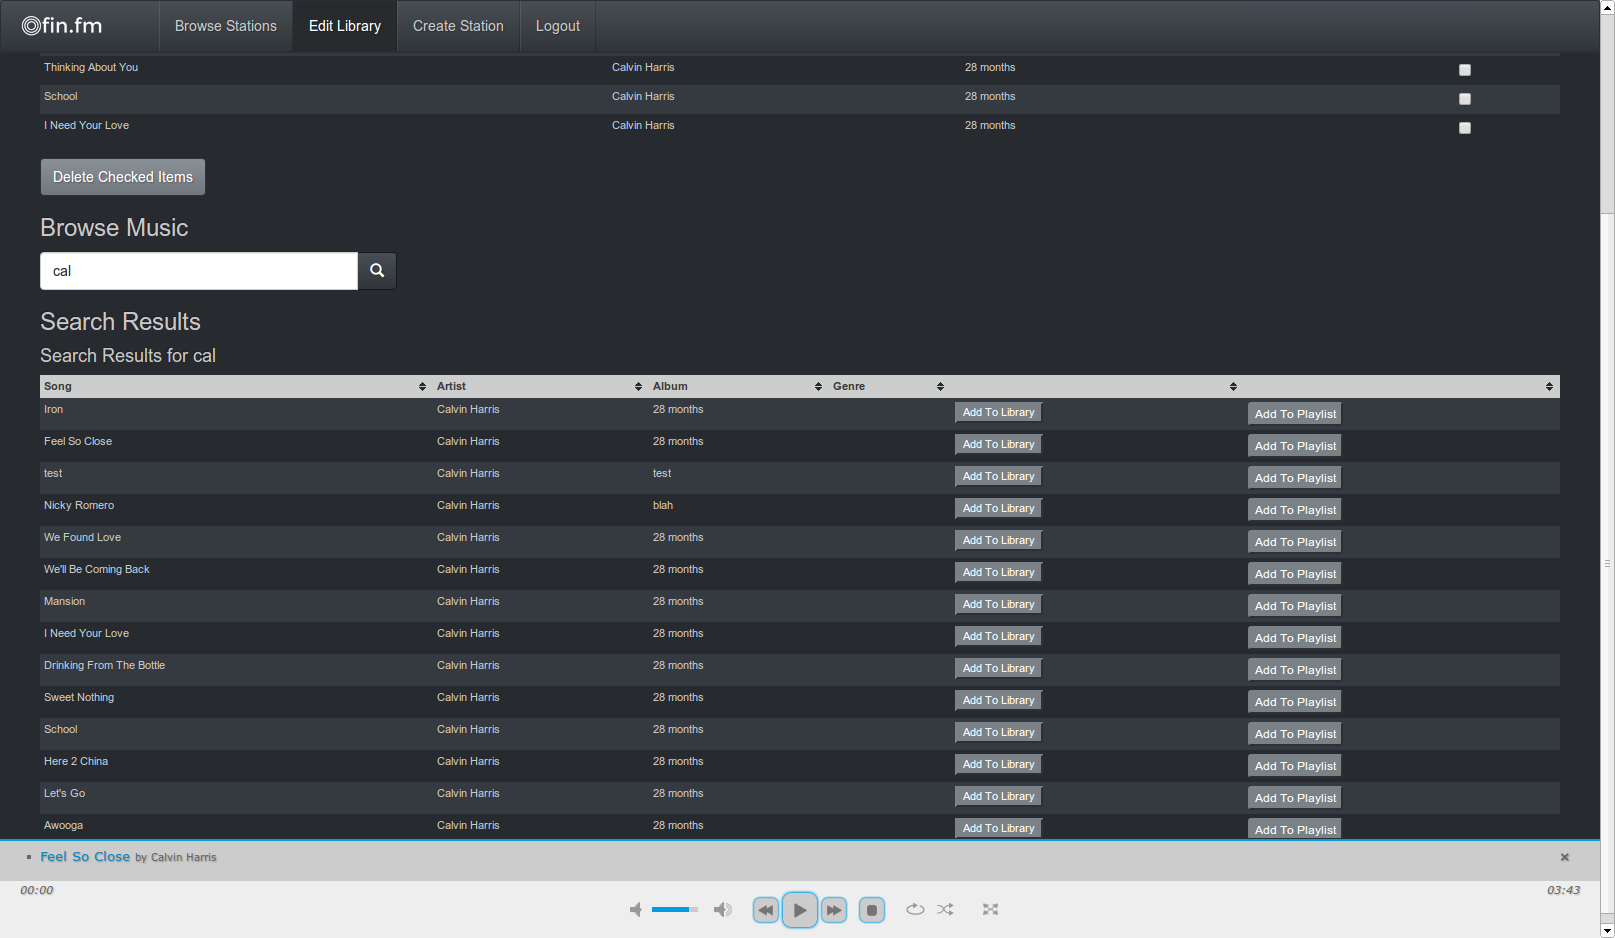
\includegraphics[width=1.0\textwidth]{screenshots/browse-library.png}
    \caption{Browsing the user curated library}
    \label{browse-library}
\end{figure}

\subsection{Vote determines playlist + Stream Page}
There were two interfaces developed for each station type. One being a control page for the owner of the station and the other a page allowing the user connected to the station to carry out the features provided to them depending on the station type. \\
The first station type available to users is the 'Vote determines playlist + Stream'. Stations of this type allow the users connected and upvote/ down vote songs. The song with the most up positive votes is then played next. This table also refreshes every second to provide the user with up-to-date information.\\

\textbf{Owners Page}: As this station is designed to give control to the connected users it was decided that this page would have limited functionality. The playlist for the station is displayed in a table format that displays the song information and either the number of votes it has received or if it has already been played. This table is automatically ordered highest number of votes to lowest. The owner may also use the controls on the media player to either skip a song, stop, or pause it. 
Users also have the option to click the 'QR Code' button in the top right corner which will generate a QR code linking to this station. This was created with the idea that stations created for events can print off the QR code and display it around the event and make it easy for users to connect to the station.
\begin{figure}[H]
  \centering
    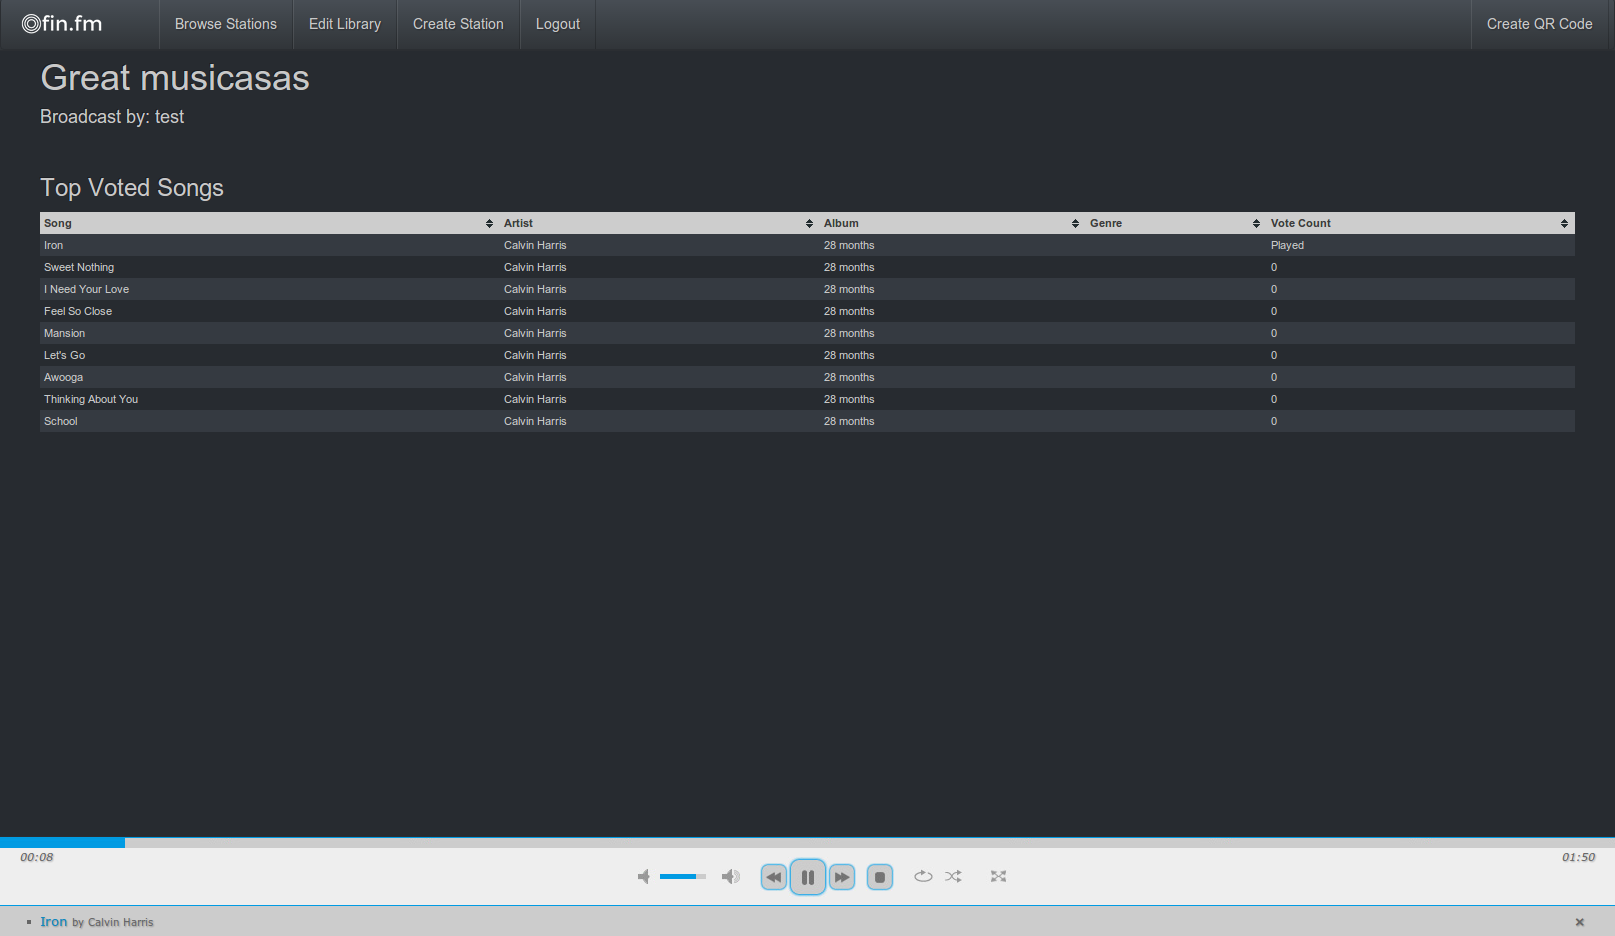
\includegraphics[width=1.0\textwidth]{screenshots/station-type-1-owner.png}
    \caption{Owner page for Vote determines playlist + Stream station}
    \label{station-type-1-owner}
\end{figure}

\textbf{Connected User Page}: As seen in figure~\ref{station-type-1-listener} the playlist of the station is displayed in a table format continuing with the consistent style of the web application. For each item in the table it has two corresponding buttons 'Vote Up' and 'Vote Down'. When these buttons are clicked they will either +1 or -1 the total number of votes for that song respectively. The buttons are then disabled to prevent users from spamming votes for a particular song. This table also refreshes every second to provide the user with up-to-date information.
The connected user can also stream the current song being played using the media player located at the bottom of the page and if they are logged in they can add the current song to their personal playlist by clicking the 'Add Current Song To Library' button located above the table.
\begin{figure}[H]
  \centering
    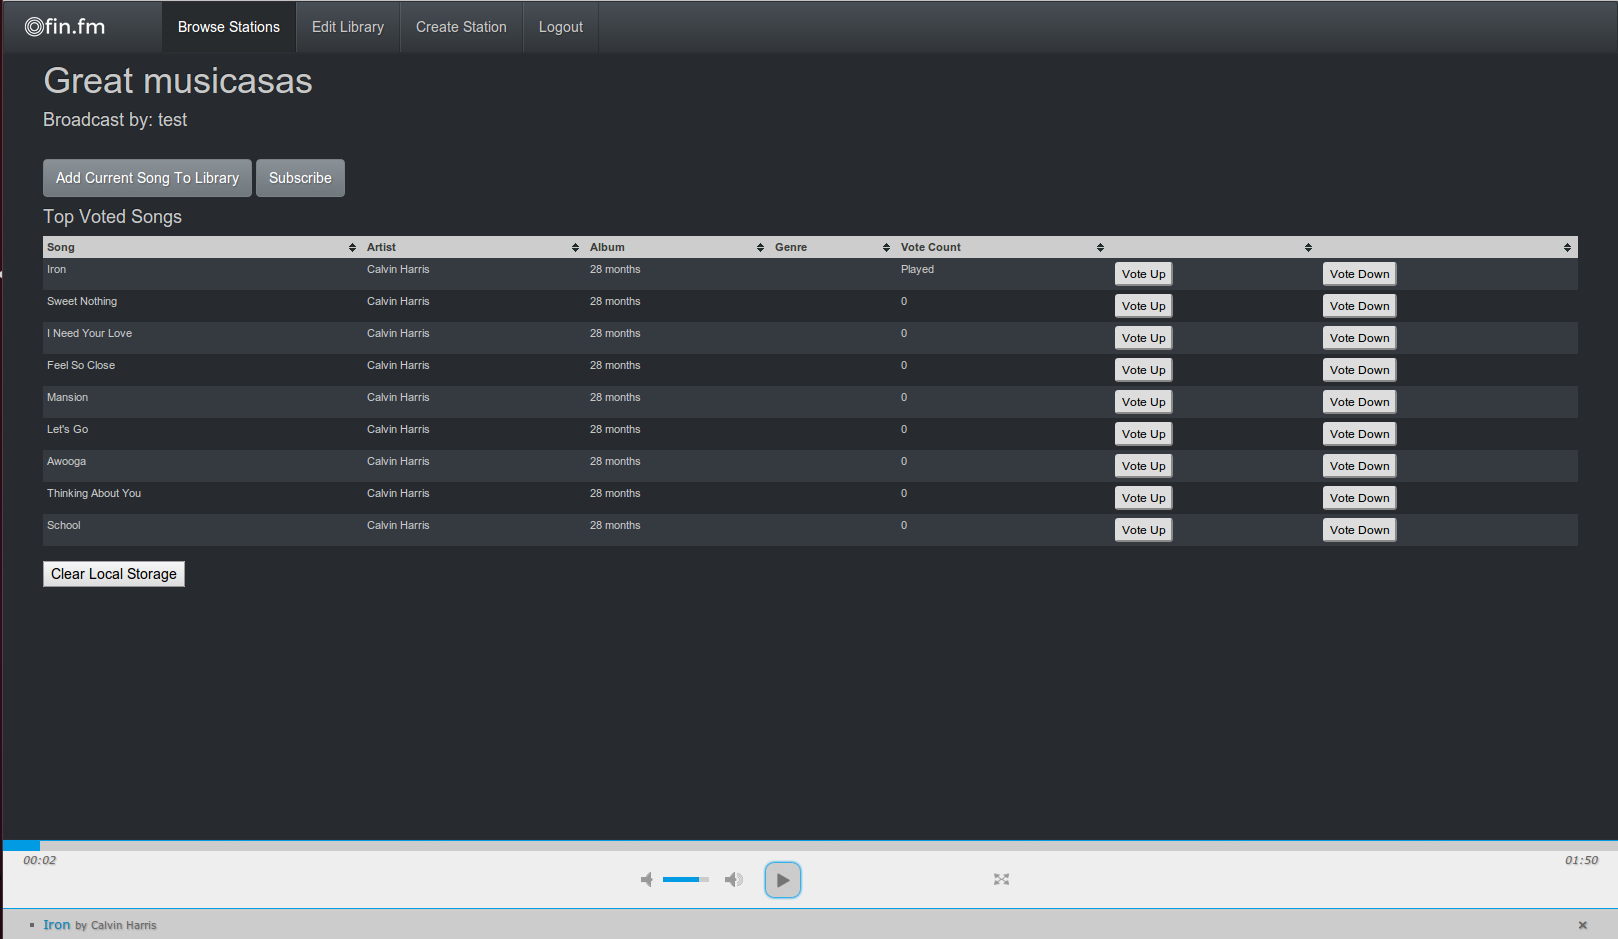
\includegraphics[width=1.0\textwidth]{screenshots/station-type-1-listener.png}
    \caption{Connected user page for Vote determines playlist + Stream station}
    \label{station-type-1-listener}
\end{figure}

\subsection{Vote determines playlist Page}
This station type is the exact same as the previous station 'Vote determines playlist + Stream' expect that connected users cannot stream the current song. This means that the owners page is the exact same as was seen previously in figure~\ref{station-type-1-owner}. The connected users page however has a few differences as seen in figure~\ref{station-type-2-listener}. Firstly because they cannot stream the current song the media play at the bottom of the page has been removed. Instead the current song is displayed to the user in a new table. Everything else is identical in functionality.
\begin{figure}[H]
  \centering
    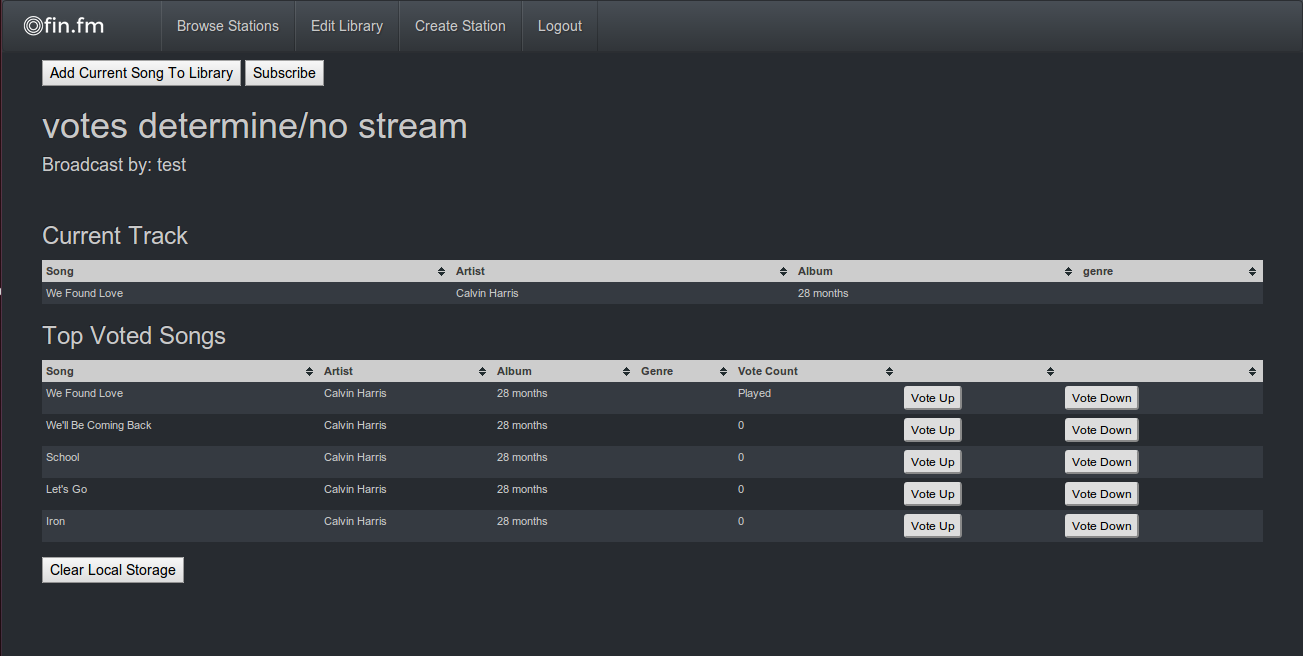
\includegraphics[width=1.0\textwidth]{screenshots/station-type-2-listener.png}
    \caption{Connected user page for Vote determines playlist station}
    \label{station-type-2-listener}
\end{figure}

\subsection{Voter feedback + Stream Page}
For this station the connected users can upvote/ down vote songs like they could in the previous two station types but the owner of the station has the final say on what song is played next.\\

\textbf{Owners Page}: This page has some similarities to the owner pages for the previous stations as it has a table displaying the playlist of the station ordered by the number of votes each song has received and a media player at the bottom of the page. The similarities stop here however as there is an extra table that displays the playlist with a button called 'Add To Playlist' for each song. When clicked the song corresponding to this button is added to a list on the right side of the page. Each item in the list can be rearranged by drag-and-drop which can bee seen in figure~\ref{drag}. Each item in this list also has two buttons. The 'Play' button will automatically play it using the media player and move it to the bottom of the list while the 'X' button will delete it from the list. Once the current song playing in the media player finishes it automatically plays the song at the top of the list and the list is then rearranged with that song now at the bottom. 
It was decided that there would be a separate table displaying the playlist with the ability to add to the list on the right instead of having that functionality in the table displaying the number of votes as this table would be constantly refreshing and changing.
\begin{figure}[H]
  \centering
    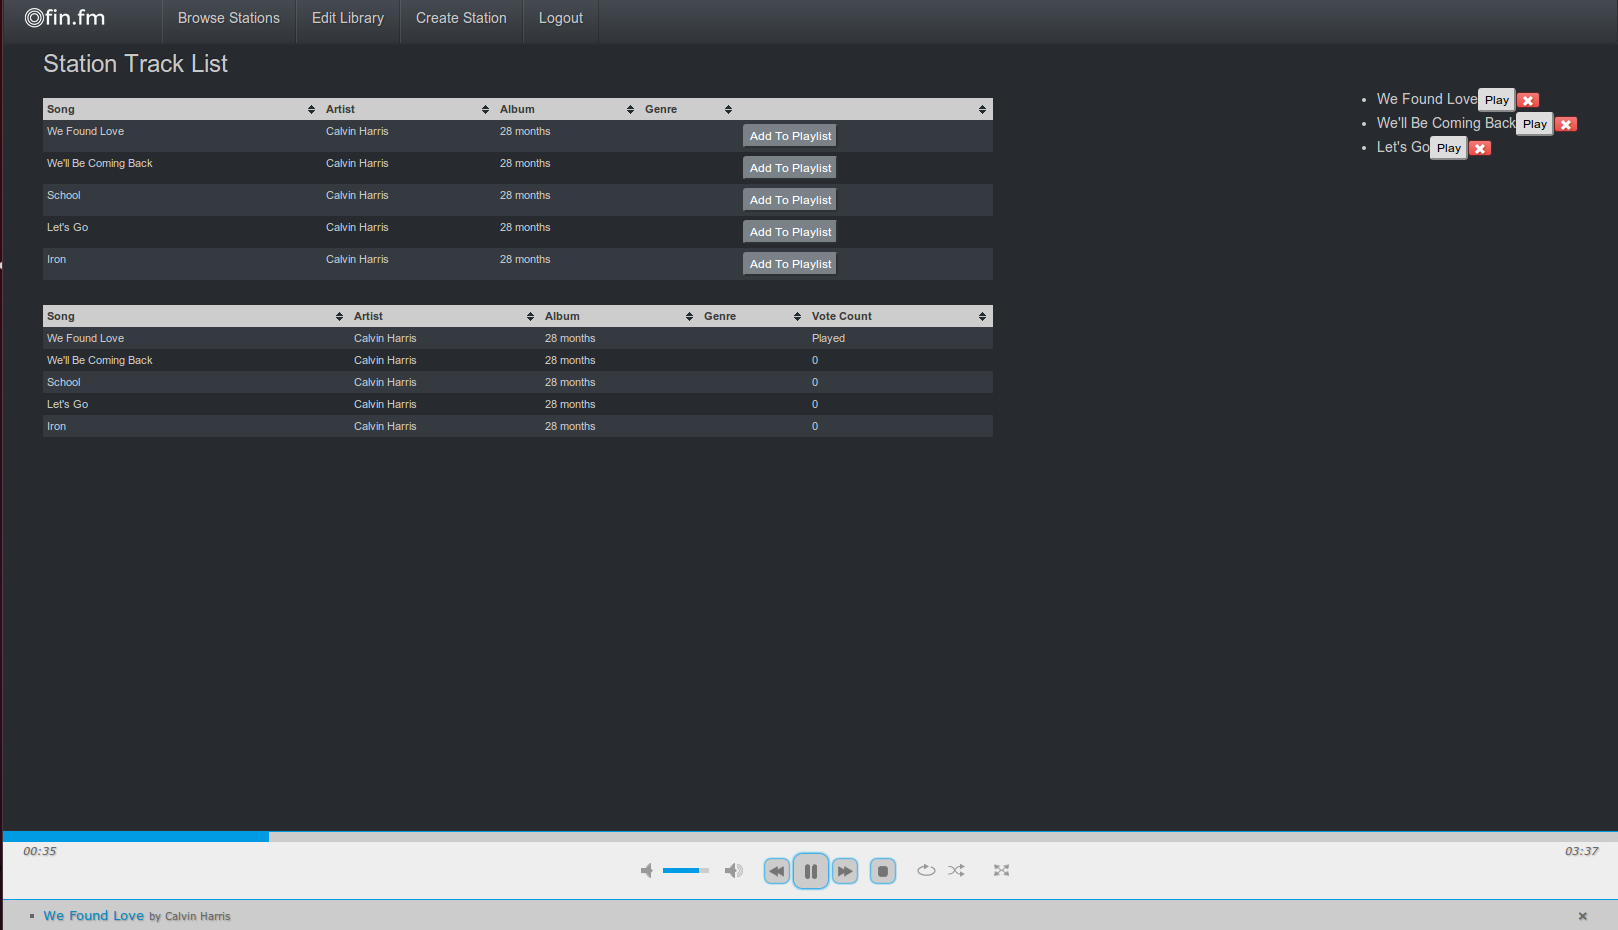
\includegraphics[width=1.0\textwidth]{screenshots/station-type-3-owner.png}
    \caption{Connected user page for Vote determines playlist station}
    \label{station-type-3-owner}
\end{figure}
\begin{figure}[H]
  \centering
    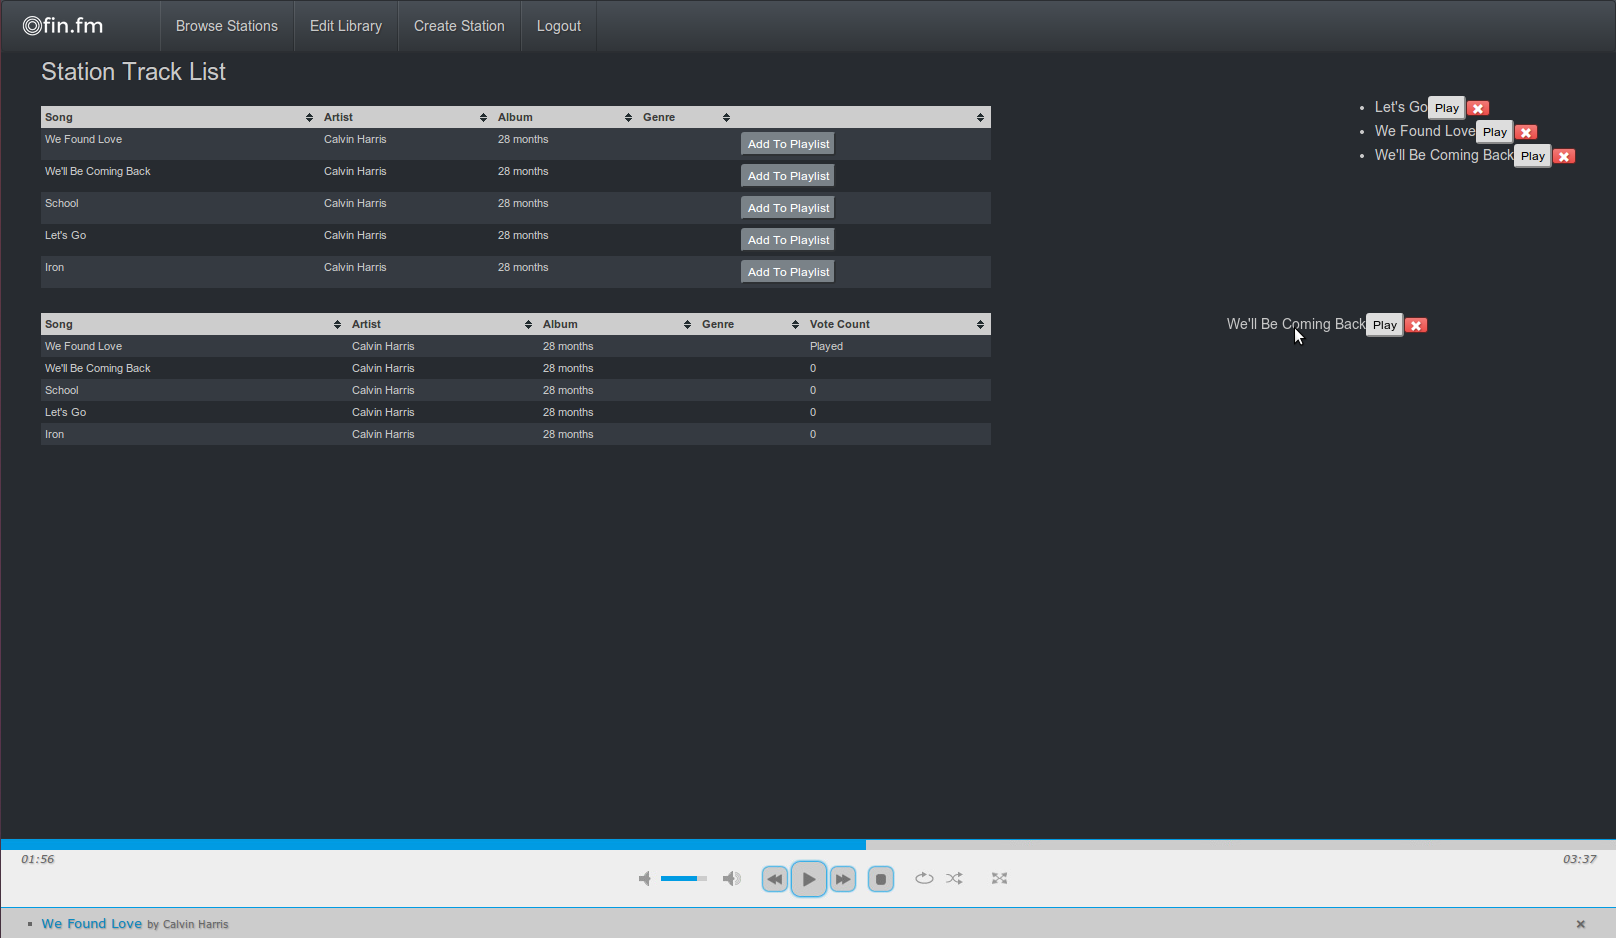
\includegraphics[width=1.0\textwidth]{screenshots/dragging2.png}
    \caption{Drag-and-Drop feature}
    \label{drag}
\end{figure}

\textbf{Connected Users Page}: This page is the exact same as the connected user page for the 'Vote determines playlist + Stream' station type seen in figure~\ref{station-type-1-listener}.

\subsection{Voter feedback Page}
This stations functionality is the exact same as the previous station with the only difference being that connected users cannot steam the current song. The connected users page is the same as seen previously in figure~\ref{station-type-2-listener}.

\subsection{Stream Page}
For the 'Stream' station type the owner has the the same control as they did in the previous two stations where they create a list using the station playlist. The user on the other hand can only stream the current song. They do not have the ability to vote for anything.\\

\textbf{Owners Page}: This page is very similar to that seen in figure~\ref{station-type-3-owner} but the table displaying the playlist ordered by the number of votes has been removed as users cannot provide any voting feedback. This can be seen in figure~\ref{station-type-5-owner}.

\begin{figure}[H]
  \centering
    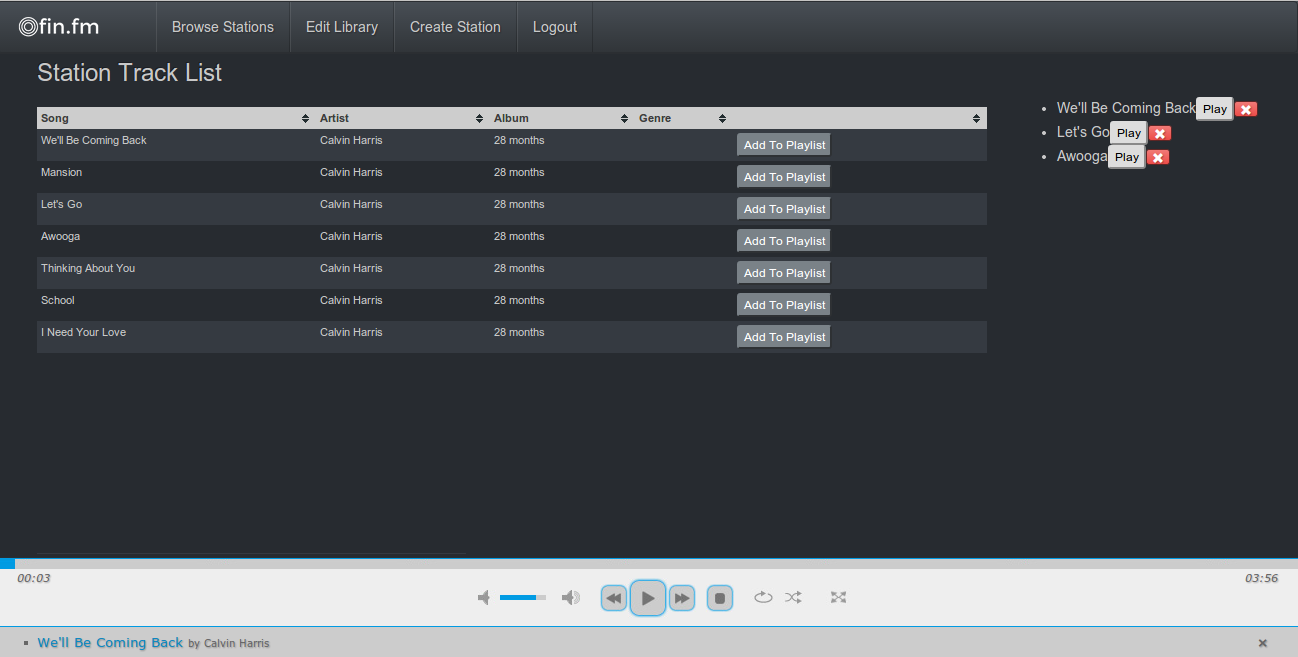
\includegraphics[width=1.0\textwidth]{screenshots/station-type-5-owner.png}
    \caption{Stream station owner page}
    \label{station-type-5-owner}
\end{figure}

\textbf{Connected Users Page}: This page is quite plain due to the lack of features. As can be seen in figure ~\ref{station-type-5-listener} the media player plays the current song and logged in users have the ability to add the current track to their library as seen previously for other stations type.

\begin{figure}[H]
  \centering
    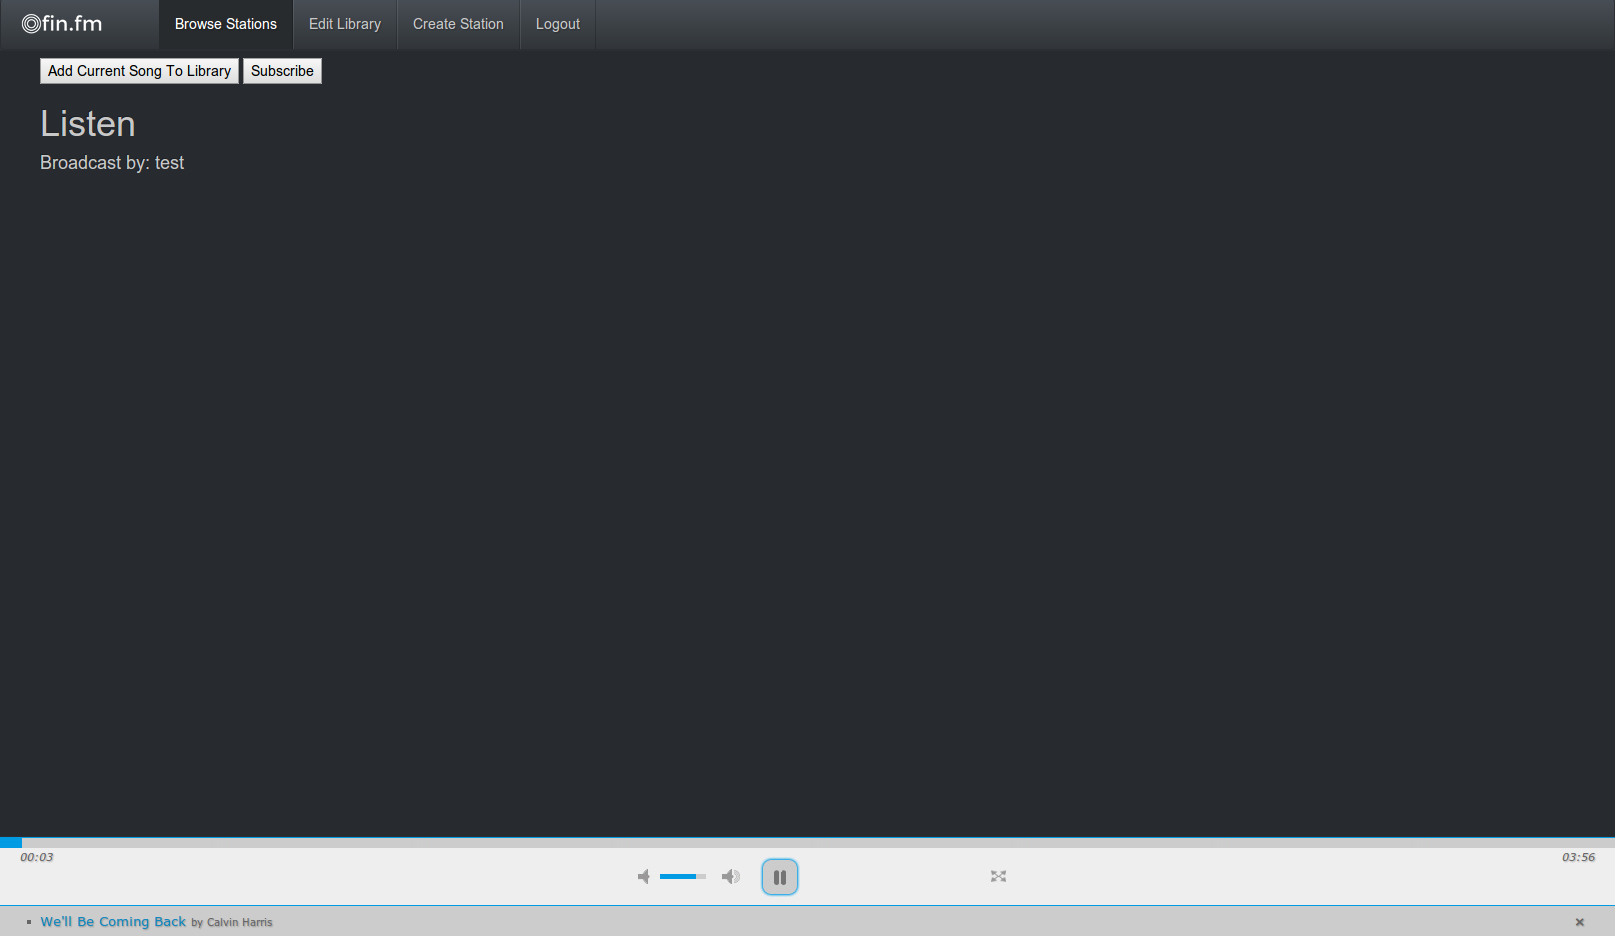
\includegraphics[width=1.0\textwidth]{screenshots/station-type-5-listener.png}
    \caption{Connected users page for stream station type}
    \label{station-type-5-listener}
\end{figure}



\chapter{Implementation}

\section{Introduction}
During this section the major parts of the implementation of the system and the issues encountered along the way will be discussed.

\section{Apache Server}
The implementation began with setting up an Apache server on a Linux machine. This was quite a simple task as a guide\cite{set_up_apache} was followed. A LAMP stack consisting of Apache, MySQL and PHP was installed and the development environment was complete. 

\section{Database Implementation}
As was stated earlier in the Research section the relational database MySQl was chosen for this project. The design and implementation of this database changed numerous times during the development process as more features were added to the project. 

\subsection{First Draft}
The first draft of the database design was carried out quite early in the project. As will be shown later this database did not cater for 
\textbf{Relational Model:}\\
Genre (Name, Summary)\\
Artist (Name)\\
Song (songId, Name, Artist)\\
Album (albumId, Title, Genre, Artist)\\
Track (trackId, Album, Song, Filepath)\\
Users (userId, Password, Username, Email)\\
Library (userId, songId)\\
Station (userId, stationId, songId)\\
StationPermisions(stationId, Password, UserPermisions)\\
\textbf{Foreign Keys:}\\
Artist (Name) -$>$ Album (Artist)\\
Artist (Name) -$>$ Song (Artist)\\
Album (Genre) -$>$ Genre (Name)\\
Album (albumId) -$>$ Track (Album)\\
Song (songId) -$>$ Track (trackId)\\
Song (Name) -$>$ Track (Song)\\
Track (trackId) -$>$ Library (songId)\\
Users (userId) -$>$ Library (userId)\\
Library (songId) -$>$ Station (songId)\\
Station (stationId) -$>$ StationPermisions (stationId)\\
\begin{figure}[H]
  \centering
    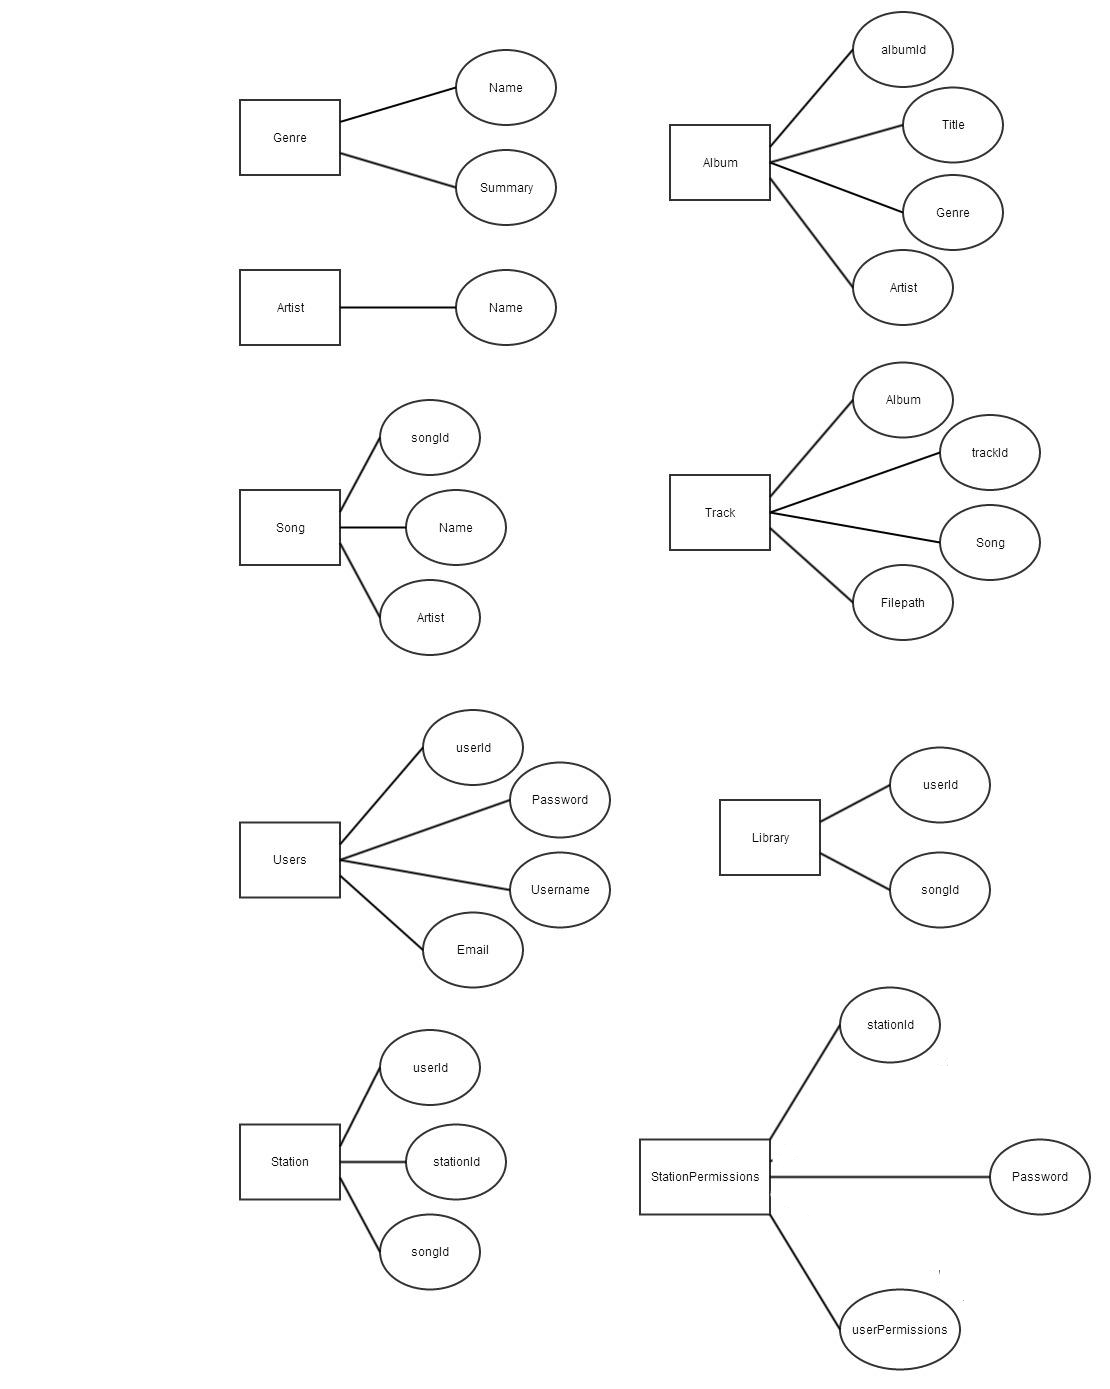
\includegraphics[width=0.7\textwidth]{screenshots/database1.png}
    \caption{The list of main entities}
    \label{database1}
\end{figure}
\begin{figure}[H]
  \centering
    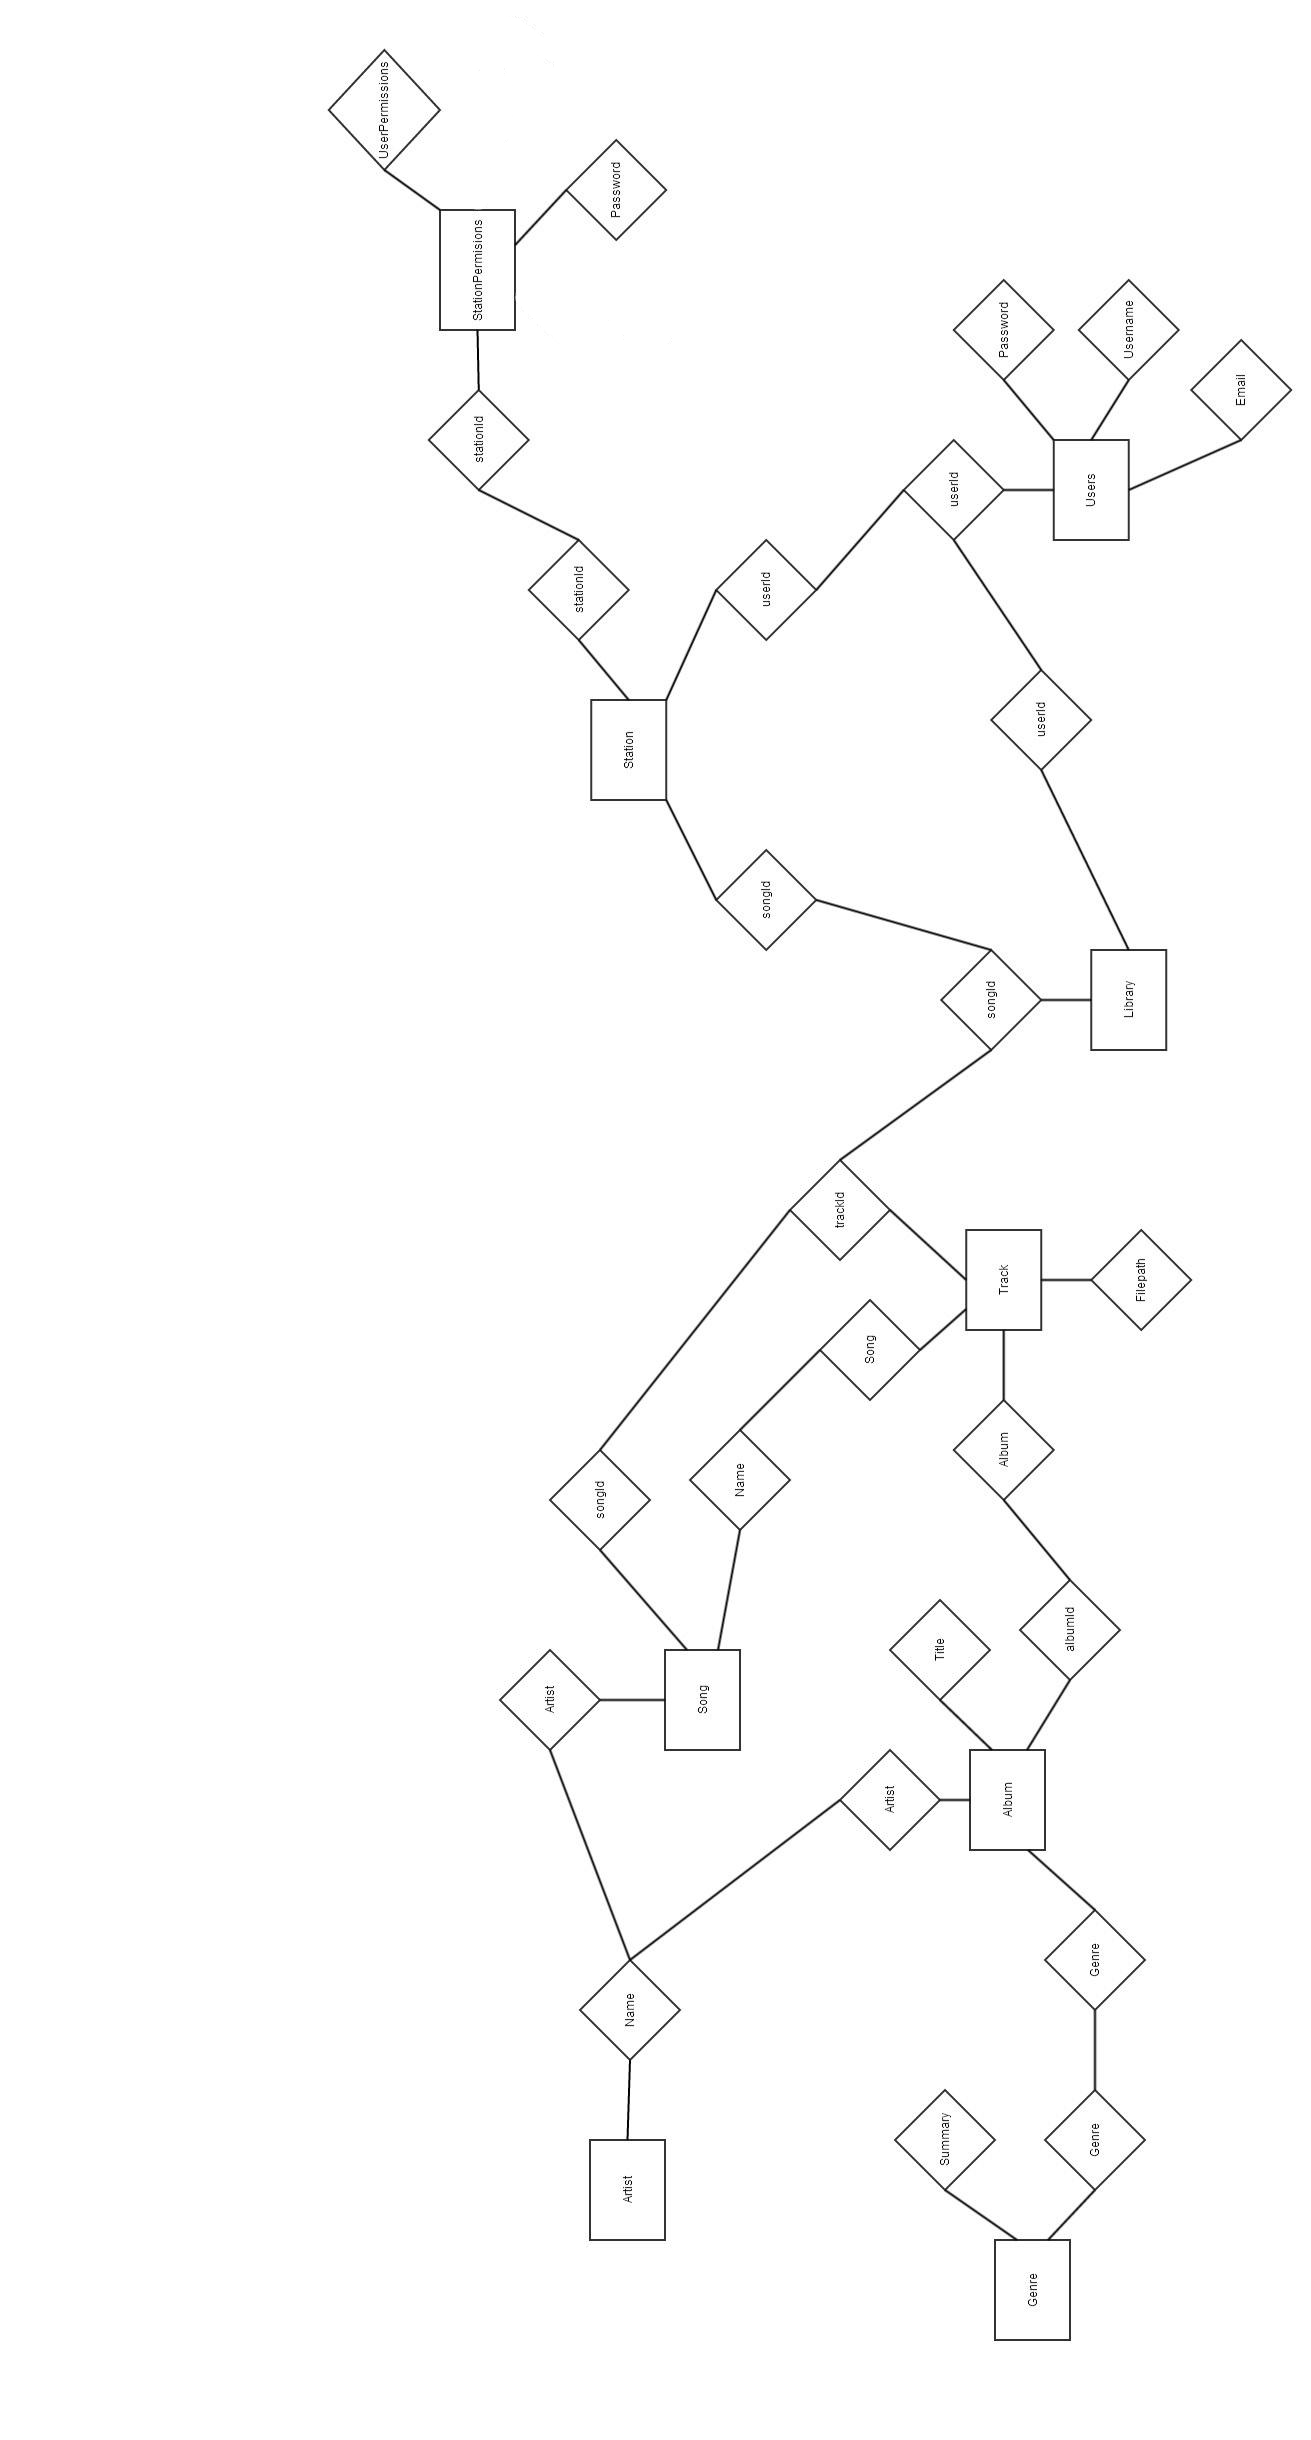
\includegraphics[width=0.8\textwidth]{screenshots/database2.png}
    \caption{The main relationships}
    \label{database2}
\end{figure}

\subsection{Final Draft}
The final draft of the database had to cater for extra features that were not planned for in the first draft. Some of these features included login security, keeping track of played songs, and knowing the current song.\\
\textbf{Relational Model:}\\
members (id, username, email, password, salt)\\
login\_attempts (user\_id, time)\\
library (userID, songID)\\
track (trackID, album, song, filepath, artist, genre)\\
stations (stationID, userID, stationName, trackList, stationType, description, genre, status, currentTrack)\\
votes (songID, stationID, voteCount, played)\\
\textbf{Foreign Keys:}\\
members (id) -$>$ login\_attempts (user\_id)\\
members (id) -$>$ library (userID)\\
members (id) -$>$ stations (userID)\\
library (songID) -$>$ track (trackID)\\
stations (stationID) -$>$ votes (stationID)\\
votes (songID) -$>$ track (trackID)\\
\begin{figure}[H]
  \centering
    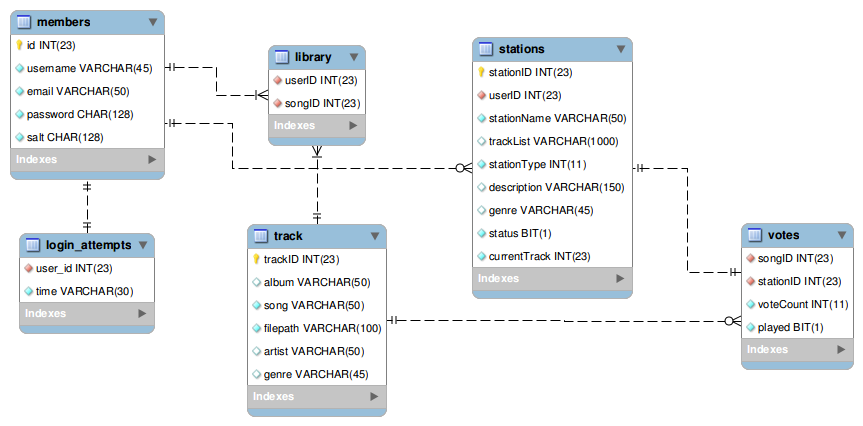
\includegraphics[width=1.0\textwidth]{screenshots/erd.png}
    \caption{ERD for final draft}
    \label{erd}
\end{figure}

\subsection{Conclusion}
Overall due to lack of experience and restrictions in time I do not feel that the final draft of the database implementation is good enough. This will be one of the sections discussed later in future work.


\section{jPlayer}
Once the development enviornment was created the next task to be tackled was finding a means of playing the audio files used in this web application. After much research and testing of the software available jPlayer\cite{jplayer} an opensource media library writen in JavaScript was chosen, this is also used by Pandora which was discussed earlier in the research section. Listing 1 below is some sample code that creates a jPlayer media player using jQuery. This example shows the correct format to use.

\begin{lstlisting}[caption=Example code to create a jPlayer media player]
	var myPlaylist = new jPlayerPlaylist({
		jPlayer: '#jquery_jplayer_N',
		cssSelectorAncestor: "#jp_container_N"
	}, [
		{
			title:"Cro Magnon Man",
			artist:"The Stark Palace",
			mp3:"http://www.jplayer.org/audio/mp3/TSP-01-Cro_magnon_man.mp3",
			oga:"http://www.jplayer.org/audio/ogg/TSP-01-Cro_magnon_man.ogg",
			poster: "http://www.jplayer.org/audio/poster/The_Stark_Palace_640x360.png"
		}
	], {
		playlistOptions: {
			enableRemoveControls: true
		},
		swfPath: "js",
		supplied: "webmv, ogv, m4v, oga, mp3",
		smoothPlayBar: true,
		keyEnabled: true,
		audioFullScreen: true
	});
\end{lstlisting}

jPlayer also provides the functionality of loading in different playlists to an existing jPlayer object. This can be done simply using a function called 'setPlaylist()'. Listings 2 is a small sample of how a playlist would be added to the jPlayer object in Listing 1.

\begin{lstlisting}[caption=Example code to add a playlist to a jPlayer object]
	myPlaylist.setPlaylist([
			{
				title:"Cro Magnon Man",
				artist:"The Stark Palace",
				mp3:"http://www.jplayer.org/audio/mp3/TSP-01-Cro_magnon_man.mp3",
				oga:"http://www.jplayer.org/audio/ogg/TSP-01-Cro_magnon_man.ogg",
				poster: "http://www.jplayer.org/audio/poster/The_Stark_Palace_640x360.png"
			},
			{
				title:"Your Face",
				artist:"The Stark Palace",
				mp3:"http://www.jplayer.org/audio/mp3/TSP-05-Your_face.mp3",
				oga:"http://www.jplayer.org/audio/ogg/TSP-05-Your_face.ogg",
				poster: "http://www.jplayer.org/audio/poster/The_Stark_Palace_640x360.png"
			}]);
\end{lstlisting}

The next step in creating the needed functionality for this project was to figure out how to dynamically create a playlist and load it into the jPlayer object. This one problem took quite a large amount of time to solve due to the limited documentation available but there was a relatively easy answer. the 'setPlaylist()' function takes a JSON array as a parameter for the playlist data. A jQuery function called jQuery.getJSON()\cite{getJSON} was found which can fetch a JSON array from a separate PHP file. Listing 3 shows a simple PHP file that creates a JSON array while Listings 4 is an example of how it could be fetched and added to a jPlayer object.

\begin{lstlisting}[caption=PHP file creating a JSON array]
	$playlist[] = array('title' => 'Feel So Close', 'mp3' => 'Feel_So_Close.mp3' );
	echo json_encode($playlist);
\end{lstlisting}

\begin{lstlisting}[caption=jQuery.getJSON() used to add playlist to jPlayer object]
	$.getJSON("createJSONarray.php",function(data){
		myPlaylist.setPlaylist(
			data
		);
	});	
\end{lstlisting}

Now that the jPlayer object playlist can be updated with a dynamically created playlist attention was turned creating a means of updating the playlist with the next top voted song once the current song had finished. The issue with limited documentation was again run into while trying to solve this problem. A event called 'jPlayer.event.ended'\cite{jPlayerFunctions} was found while doing research on the problem. This event is used to bind the song ending event to different button in the jPlayer object as can be seen in Listing 5.

\begin{lstlisting}[caption=Example for jPlayer.event.ended]
$("#repeat-on").click( function() {
  $("#jpId").bind($.jPlayer.event.ended + ".jp-repeat", function(event) { // Using ".jp-repeat" namespace so we can easily remove this event
    $(this).jPlayer("play"); // Add a repeat behaviour so media replays when it ends. (Loops)
  });
  return false;
 });
\end{lstlisting}

After spending a large amount of time I was unable to to solve the problem of updating the playlist with the next top voted song once the current song had finished using this event and was forced to explore different means. While exploring new options a HTML5 Media Event\cite{inspector} Inspector was discovered. This software displays a table showing every jPlayer event and notifies when they are triggered. The decision was made to go through the code\cite{inspector-code} for this and figure out how they used the 'jPlayer.event.ended' event. 

While going through this code it was discovered that the code in Listing 6 goes through each function. The next step was trying to extract the useful parts of the code and modify them to solve the problem at hand. This however turned out to be far too time consuming and after a couple weeks it was decided that too much time was already spent on this and a more simplistic would be implemented. 

\begin{lstlisting}[caption=Function in Inspector used to go through events]
$.each($.jPlayer.event, function(eventName,eventType) {});
\end{lstlisting}

This more simplistic means used the Inspector code as it was but just added in a command for when the 'jPlayer.event.ended' event was triggered.\\
The final implementation used for solving the issue at hand went as follows : 
\begin{enumerate}
\item Once a 'jPlayer.event.ended' event was triggered the text within a hidden div was changed to 'change' using jQuery.
\item This change in text would then trigger a jQuery function which would fetch a JSON array containing a the details of the next top voted song for this station.
\item Once this JSON array was received it was then added to the the jPlayer object using the 'setPlaylist()' function. 
\end{enumerate}
Listing 7 shown bellow is a snippet of code which shows how step 1 was carried out. This was implemented in the Inspector source code where it goes through each event that is fired. Unfortunately this is a poor and inefficient means of solving the problem but was the only option due to time constraints.
\begin{lstlisting}[caption=Updating div when 'ended' event is triggered]
$.each($.jPlayer.event, function(eventName,eventType) {
				config.eventJq[eventType] = $("#" + config.eventId[eventType]);
				config.eventJq[eventType].text(eventName + " (" + config.eventOccurrence
				[eventType] + ")"); // Sets the text to the event name and (0);
				
				config.jPlayer.bind(eventType + ".jPlayerInspector", function(e) {
					
					if (eventName == 'ended'){
						$("#songEndTrigger").val("change").trigger('change');
					}	
\end{lstlisting}
Steps 2 and 3 are carried out in the code shown in Listing 8 displayed below. 
\begin{lstlisting}[caption=Fetches the playlist containing the next top voted song]
//Updates playlist when song has ended
	$( "#songEndTrigger" ).change(function() {
		$.getJSON("getNextTopVotedSong.php?stationID="+stationID,function(data){
			myPlaylist.setPlaylist(
				data
			);
		});
	});
\end{lstlisting}

\section{Voting System}
this section covers the up voting and down voting of songs by users connected to a station. During planning there were a few different possible options that were contemplated. The first involved users having to be signed in if they were to vote on songs. Voting information would then be stored in the database which would prevent spamming of votes for a song. This method however did not fit in with the project as a user at a bar or a social event would more than likely not go to the effort of registering for the service. 
As non registered users should have the ability to vote the voting history by that user must be stored locally in order to prevent spamming of votes. For this there were two options, either cookies\cite{cookies} or local storage\cite{LS} could be used.\\
\textbf{Cookies}\\
Pros:
\begin{itemize}
 \item Legacy support.
 \item Persistent data.
 \item Expiration dates.
\end{itemize} 
Cons:
\begin{itemize}
\item Cookies are stored in a single string which can make parsing data difficult.
\item Data is unencrypted.
\item Sent with every HTTP request.
\item Limited to 4KB in size.
\item SQL injection attacks can be carried out with cookies.
\end{itemize}
\vskip1cm
\textbf{Local Storage}\\
Pros:
\begin{itemize}
 \item Persistent data stored locally in browser.
 \item Is not sent in every HTTP request.
 \item 5120KB in size.
\end{itemize} 
Cons:
\begin{itemize}
\item Not supported by older browsers.
\end{itemize}
\vskip1cm
After looking at the pros and cons for each option Local storage was chosen over Cookies. The main reasons for this choice was the significant size advantage of data that could be stored and the fact that the information is not sent with every HTTP request. The only downfall to using this system is that it will not work for devices with cookies disabled. Listing 9 shows the jQuery function used to disable the buttons for previously voted songs when the page is loaded.

\begin{lstlisting}[caption=Disabling buttons for previously voted songs]
$( document ).ready(function() {
	var data = localStorage.getItem("SONGID");
	var arr = data.split(':');
	for( var i = 0; i <= arr.length; i++){
		var buttonID = arr[i];
		$("#" + buttonID + ".upVoteButton").prop("disabled", true);
		$("#" + buttonID + ".downVoteButton").prop("disabled", true);
	}		
});
\end{lstlisting}

Keeping track of the votes for each song was a relatively easy task. As seen earlier in database implementation shown in Figure~\ref{erd} there is a field named 'voteCount' for each song in a station . This field contains an int value which starts at 0. When either the 'vote up' or 'vote down' button is clicked this value 'voteCount' is either incremented +1 or decremented -1.

\section{Register and Login System}
There was a huge number of different Register and Login System examples available online but most of these were insecure in one way or another. These systems can be vulnerable to a numerous attacks and while designing a system one should try to defend against the following list of attacks:
\begin{itemize}
\item SQL Injections.
\item Session Hijacking.
\item Network Eavesdropping.
\item Cross Site Scripting. 
\item Brute Force Attacks.
\end{itemize} 
To defend against all these attacks an approach that uses data filtering and encryption is used. The first step to creating a secure register and login system is to create tables in the MySQL database to hold user information. The first table created holds the user information which can be seen in Listing 10. 
\begin{lstlisting}[caption=Code used to create the members table]
CREATE TABLE `members` (
    `id` INT NOT NULL AUTO_INCREMENT PRIMARY KEY,
    `username` VARCHAR(30) NOT NULL,
    `email` VARCHAR(50) NOT NULL,
    `password` CHAR(128) NOT NULL,
    `salt` CHAR(128) NOT NULL 
)
\end{lstlisting}
For added security the members table stores the password as a one way hash using a salt value. This means that if any malicious users gains access to your database they wont learn all the users passwords as they are not stored in plain text.

The next table to be created is a login attempts table. This tables main function is to make brute force attacks more difficult for malicious users. 
\begin{lstlisting}[caption=Code to create login attempts table]
CREATE TABLE `login_attempts` (
    `user_id` INT(11) NOT NULL,
    `time` VARCHAR(30) NOT NULL
)
\end{lstlisting}

Once these are created a function to check for Brute Force attacks must be created. A brute force attack is carried out by trying many common passwords against a single email address. For example trying the password 123. In the function shown in Listing 12 failed login attempts over the previous 2 hours are counted. If there are more than 5 failed login attempts for an account within those 2 hours the account is temporarily blocked.
\begin{lstlisting}[caption=Brute Force prevention function]
function checkbrute($user_id, $mysqli) {
    // Get timestamp of current time 
    $now = time();
 
    // All login attempts are counted from the past 2 hours. 
    $valid_attempts = $now - (2 * 60 * 60);
 
    if ($stmt = $mysqli->prepare("SELECT time 
                             FROM login_attempts <code><pre>
                             WHERE user_id = ? 
                            AND time > '$valid_attempts'")) {
        $stmt->bind_param('i', $user_id);
 
        // Execute the prepared query. 
        $stmt->execute();
        $stmt->store_result();
 
        // If there have been more than 5 failed logins 
        if ($stmt->num_rows > 5) {
            return true;
        } else {
            return false;
        }
    }
}
\end{lstlisting}
The next attack to defend against is session hijacking. To do this a function is used that takes sessions variables and hashes them with users browser data using a sha512 one way hash. 
Now the registration page is created. To make the users register information as secure as possible it must pass a certain set of criteria which are:
\begin{itemize}
\item Usernames may contain only digits, upper and lower case letters and underscores.
\item Emails must have a valid email format.
\item Passwords must be at least 6 characters long.
\item Passwords must contain:
\begin{itemize}
\item At least one upper case letter (A..Z)
\item At least one lower case letter (a..z)
\item At least one number (0..9)
\end{itemize}
\end{itemize}

\section{Edit Station Page}
As stated previously in the design section and seen in Figure\ref{edit-station} the page must be dynamic and display the form already filled in with the data previously selected, jQuery was chosen to fulfil this task. 
The form itself consists of a table displaying each song in the users personal library along with a corresponding check box. There are also 2 input fields which take String values for the station name and description, along with a select menu for the genre and radio buttons for the station type. The following it a Listing containing the jQuery code used to populate this form.\\
\begin{lstlisting}[caption=Populate edit library form]
$(document).ready(function(){
	var stationID = $("#stationID").text();
	//CHECKING CHECKBOXES IF THEY ARE ALREADY IN STATION
	$.getJSON("getStationSongIDs.php?stationID="+stationID,function(data){
		var songIDs = data;
		$('input[type=checkbox]').each(function () {
			if(jQuery.inArray($(this).val(),songIDs) != -1){
				$("input:checkbox[value="+$(this).val()+"]").attr("checked", true);
			};		
		});
	});
						
	//SETTING FORM VALUES 
	$.getJSON("getStationDetails.php?stationID="+stationID,function(data){
		$('#stationName').val(data[0]);
		$('#' + data[1]).prop('checked',true);
		$('#stationDescription').val(data[2]);
		$('#genre').val(data[3]);				
	});
}); 
\end{lstlisting}
Both PHP files called in the jQuery functions are basic files that fetch required data from the database and return it in a JSON array that can be processed. snippets from these PHP files can be seen in Listings 14 and 15 below.\\
\begin{lstlisting}[caption=Snippet of code from getStationSongIDs.php]
$stationID = $_GET['stationID'];
$playlist = array();
$result = mysqli_query($con,"SELECT songID FROM votes WHERE stationID = {$stationID};");
if (!$result) {
    	printf("Error: %s\n", mysqli_error($con));
	exit();	
}
	
while($row = mysqli_fetch_array($result)){
	$playlist[] = $row['songID'];
}

echo json_encode($playlist);
}); 
\end{lstlisting}
\begin{lstlisting}[caption=snippet of code from getStationDetails.php]
$stationID = $_GET['stationID'];
$playlist = array();
  $result = mysqli_query($con,"SELECT * FROM stations WHERE stationID = {$stationID};");
if (!$result) {
    	printf("Error: %s\n", mysqli_error($con));
   	 exit();	
}
	
while($row = mysqli_fetch_array($result)){
	$playlist[] = $row['stationName'];
	$playlist[] = $row['stationType'];
	$playlist[] = $row['description'];
	$playlist[] = $row['genre'];
}

echo json_encode($playlist);
\end{lstlisting}

\chapter{Testing and Evaluation}

\section{Introduction}
In order to produce the best possible project rigorous testing is required and the extent of this testing is a crucial factor in determining if it was a success or failure. This chapter will discuss the various testing techniques used and the results gathered from them where possible. 

\section{Unit Testing}
Unit testing is a software development process in which the smallest testable parts of an application, called units, are individually and independently scrutinised for proper operation\cite{unit-testing}.This the main method of testing code.  For example, every time new jQuery functions were added to the project or new  these new parts of code had to be adequately tested. Once all of the units in a program had been found to be working in the most efficient and error-free manner possible, larger components of the program were be evaluated by means of integration testing.

\section{Integration Testing}
For integration testing the units used in unit testing were grouped together to expose defects in the interfaces and in the interactions between integrated components of the project. 

An example of an integration test would be combining two unit tests, one unit test tests whether a class correctly connects to a database and retrieves the data correctly. The would be a test to test whether an interface correctly displays information from the class it is connected to. In this case the integration test would test whether the retrieval of information from the database, and the displaying of this information within the interface, operates smoothly and as intended.

\section{Usability Testing}
This testing was carried out when the main features of the project were completed. For this two different questionnaires were created and handed out to two different groups. The first group consisted of students who agreed to use this web application at social gatherings they were hosting. The second was a group consisting of managers and promoters of local pubs and clubs. 

\subsection{Students}
To get feedback from students this questionnaire was handed out to a total of 25 students at 2 separate gatherings.\\
\textbf{Questionnaire}
\begin{enumerate}
\item What was your favourite feature of the web application and why?
\item What was your least favourite feature of the web application and why?
\item Was the design and layout of the web application easy to understand?
\item Was it easy to interact with the web application?
\item Would you use this web application again and if so when?
\item What would you add to improve the application?
\end{enumerate}
\textbf{Questionnaire Results}
\begin{enumerate}
\item What was your favourite feature of the web application and why?
\begin{itemize}
\item Almost every user selected the creating a station where the next played song is decided on the number of votes it has received.
\end{itemize}
\item What was your least favourite feature of the web application and why?
\begin{itemize}
\item There was no stand out feature that users did not like however one user said they would prefer a drag and drop interface instead of check boxes for the 'Create Station' page.
\end{itemize}
\item Was the design and layout of the web application easy to understand?
\begin{itemize}
\item Here, the vast majority of users were happy with the design and layout. Many commented on how modern and clean it looked. Some users however did not quite understand the term 'station'
\end{itemize}
\item Was it easy to interact with the web application?
\begin{itemize}
\item Yet again most users were perfectly happy but there were multiple comments of clicking the 'upvote' and 'down vote' buttons on their mobile devices did not register first try.
\end{itemize}
\item Would you use this web application again and if so when?
\begin{itemize}
\item Every user said they would use it again and the most popular setting would be the same as they were in, a social gathering at a friends house. Many also stated that they would like to see it implemented in bars and clubs. One user also stated that it could be used at gigs to help a band determine their setlist.
\end{itemize}
\item What would you add to improve the application?
\begin{itemize}
\item A lot of users were happy with the provided features but quite a few stated that they would like to be able to connect it to their Youtube, Spotify and Grooveshark accounts and access music from their. Another popular added feature would be to suggest songs to the owner of the station.
\end{itemize}
\end{enumerate}

\subsection{Bar/Club Managers and Promoters}
This questionnaire was handed out to Mr. Steven Randles who opened the nightclub Beta and now manages The Savoy nightclub, and Mr. Mark Stanton who is a promoter for The Holy Cow bar and The Bowery nightclub. 
\textbf{Questionnaire}
\begin{enumerate}
\item What was your favourite feature of the web application and why?
\item What was your least favourite feature of the web application and why?
\item Do you believe that this web application could be used as part of your business?
\item What would you add to improve the application?
\end{enumerate}
\textbf{Questionnaire Results}
\begin{enumerate}
\item What was your favourite feature of the web application and why?
\begin{itemize}
\item Both Stephen and Mark agreed that the feature of creating a station where the next played song is decided on the number of votes it has received was their favorite as it was completely different to anything they had seen before.
\end{itemize}
\item What was your least favourite feature of the web application and why?
\begin{itemize}
\item Neither felt like any other the features were bad and that all were essential to the web application.
\end{itemize}
\item Do you believe that this web application could be used as part of your business?
\begin{itemize}
\item Mark was very positive to the idea of this being used in the establishments he promotes. Stephen on the other hand was slightly apprehensive as he felt like established DJ's may not be happy with it. 
\end{itemize}
\item What would you add to improve the application?
\begin{itemize}
\item Both Mark and Stephen agreed that that adding functionality to support Youtube, Spotify and other services would improve the application. Stephen also felt that working closely with professional DJ's would help add features such a displaying songs with certain beats per minute at a certain time. 
\end{itemize}
\end{enumerate}
\section{Conclusion}
Due to the testing carried out in this chapter the project was thoroughly analysed and improved to the point where it was functioning to a satisfactory level. The most popular feature was found to be creating a station where the next played song is decided on the number of votes it has received, while almost everone felt like there were many more features to be added such as integration with existing services like Youtube and Spotify. 

Also thanks to this testing both Stephen Randles and Mark Stanton decided to host events in their respective venues using this web application in the near future.

\chapter{Conclusion}

\section{Project Conclusion}
The project was incredibly enjoyable to work on. Along the way I was driven by the fact that it was a project that I had thought up of on my own and the prospect of it actually being used in pubs, clubs and social events I attend. \\
There were several aspects of the implementation however that I was not completely satisfied with. As mentioned previously the means of updating the media player when a song ends is not implemented well enough and the database design is also not completely up to scratch.\\
Overall I feel the project was a success and having a working web application with most almost all of the functionality I had set out to achieve is extremely satisfying. \\

\section{Personal Conclusion}
Overall, I am pleased with the my own performance and dedication during this project and learning outcomes. As I am studying the 'Web Stream' part of the computer science degree I felt it was important for me to take on a project which was heavily based on the web. I had knowledge in web development due to freelance work in the past but I had never created anything this complex. \\
From creating a safe and secure web application, to working with multiple data types as well as drastically improving my jQuery skills I am incredibly pleased with what I have learnt due to this project.\\
I am disappointed with some aspects of the project however with the means of updating the media player when a song ends was the main one and I feel as if I had more time I would definitely implement this in an elegant way.\\
The project as a whole I feel was a success and hearing that businesses want to use this project was amazing to hear.  

\chapter{Future}
This chapter contains some of the changes and inclusions of technologies that could be implemented in the future.

\section{Setting Stations To Be Live}
Currently when a user decides to make a station 'live' and allow users to connect it simply updates a bit value to 1 in the database, and when a user decides to close the browser window containing this station it then sets the bit back to 0. This was a poor implementation and I would have liked to have rectified this if I had time. However in the future I would like to implement this using sessions so that it does not rely on the user to close the window to change the state of the station. Instead the stations status is based on this session which updates the status field with a time. If this session finishes it will not update this time value, with this live stations would be displayed on the homepage if the time value in the database is within for example 3 minutes of the current time. 
 
\section{Support for Youtube, Spotify and Grooveshark Files}
The feature I would like to add to the project the most would be to integrate it with Youtube, Spotify and Grooveshark. This would involve allowing users to synch their accounts on the other services and use these library’s as sections of their own personal library. Currently there is an API called tinysong\cite{tinysong} which is available. This API allows you to access users to retrieve data from Grooveshark including songs. Spotify also has a similar API called Metadata API\cite{spotifyAPI} which allows users to explore the Spotify music catalog and retrieved track, album and artist data.

I believe all the tools are available to create this feature, and that it would add so much more to this project.

\section{Creating a JRE For File Uploads}
Currently a user can only upload files through a PHP form. This is a slow system for uploading and requires users to enter in large amounts of data for each song. Grooveshark has a great feature for uploading tracks where it uses a JRE to browse your machine\cite{jre}. This is a much better way for uploading songs and would encourage users to upload more music and contribute to the user-curated library that everyone can access.

\clearpage
\begin{thebibliography}{9}
\bibitem{apache}
Apache HTTP Server \emph{ http://en.wikipedia.org/wiki/Apache\_HTTP\_Server}

\bibitem{MySQL}
MySQL review \emph{http://www.itcentralstation.com/}

\bibitem{php}
PHP \emph{http://en.wikipedia.org/wiki/Php}

\bibitem{javascript}
JavaScript \emph{http://en.wikipedia.org/wiki/JavaScript}

\bibitem{jquery}
jQuery \emph{http://en.wikipedia.org/wiki/Jquery}

\bibitem{jplayer}
jPlayer \emph{http://jplayer.org/}

\bibitem{grooveshark}
Grooveshark \emph{ http://www.grooveshark.com} 

\bibitem{8tracks}
8tracks \emph{ http://www.8tracks.com} 

\bibitem{soundcloud}
Soundcloud \emph{ http://www.soundcloud.com} 

\bibitem{Spotify}
Spotify \emph{ http://www.spotify.com} 

\bibitem{pandora}
Pandora \emph{ http://www.pandora.com}

\bibitem{waterfall}
The Waterfall Method \emph{http://istqbexamcertification.com/what-is-waterfall-model-advantages-disadvantages-and-when-to-use-it/}

\bibitem{prototype}
The Prototyping Method \emph{http://istqbexamcertification.com/what-is-prototype-model-advantages-disadvantages-and-when-to-use-it/}

\bibitem{spiral}
The Spiral Method \emph{http://istqbexamcertification.com/what-is-spiral-model-advantages-disadvantages-and-when-to-use-it/}

\bibitem{agile}
The Agile Method \emph{http://istqbexamcertification.com/what-is-agile-model-advantages-disadvantages-and-when-to-use-it/}

\bibitem{RDSM}
Relational database \emph{http://searchsqlserver.techtarget.com/definition/relational-database}

\bibitem{top5RDSM}
Top 5 relational database \emph{http://www.thegeekstuff.com/2010/03/top-5-best-databases/}

\bibitem{RDSM-ranking}
Relational database rankings \emph{http://db-engines.com/en/ranking}

\bibitem{oracle}
Oracle review \emph{http://www.itcentralstation.com/}

\bibitem{PostgreSQL}
PostgreSQL review \emph{http://www.itcentralstation.com/}

\bibitem{microsoftSQl}
Microsoft SQL server review \emph{http://www.zdnet.com/sql-server-2012-3040155019/}

\bibitem{web_arch}
Website Architecture \emph{ http://www.wikipedia.org/wiki/Website\_architecture}

\bibitem{IA_101}
Information Architecture 101 \emph{http://sixrevisions.com/usabilityaccessibility/information-architecture-101-techniques-and-best-practices/}

\bibitem{fallback_css_js}
Fallback methods for CSS and JS \emph{http://www.hongkiat.com/blog/css-javascript-fallback-methods/}

\bibitem{web_design_conventions}
Web Design Conventions \emph{http:netaccountant.net/website-design-for-accountants/web-design-conventions/}

\bibitem{set_up_apache}
How to set up Apache on Linux \emph{https://www.digitalocean.com/community/articles/how-to-install-linux-apache-mysql-php-lamp-stack-on-ubuntu}

\bibitem{apache_stream_media}
How to stream media on Apache \emph{http://swimminginthought.com/streaming-mp4-video-webserver-solved/}

\bibitem{icecast}
Icecast Streaming \emph{http://www.icecast.org/}

\bibitem{stream_playlist}
Streaming a playlist using icecast \emph{http://www.tldp.org/HOWTO/MP3-HOWTO-11.html}

\bibitem{getJSON}
jQuery getJSON function \emph{http://api.jquery.com/jquery.getjson/}

\bibitem{jPlayerFunctions}
List of jPlayer API functions \emph{http://jplayer.org/latest/developer-guide/}

\bibitem{inspector}
HTML5 Media Event Inspector \emph{http://www.html5audio.org/2012/05/jplayers-inspector-shows-when-javascript-events-are-triggered.html}

\bibitem{inspector-code}
jPlayer Inspector Code \emph{http://www.jplayer.org/latest/js/jquery.jplayer.inspector.js}

\bibitem{cookies}
Cookies \emph{http://en.wikipedia.org/wiki/HTTP\_cookie}

\bibitem{LS}
Local Storage \emph{http://en.wikipedia.org/wiki/Web\_storage\#Local\_and\_session\_storage}

\bibitem{cookiesvsLS}
Cookies VS Local Storage \emph{http://stackoverflow.com/questions/16855680/are-there-any-drawbacks-to-using-localstorage-instead-of-cookies}

\bibitem{login-example}
Login and Register System Example \emph{http://www.wikihow.com/Create-a-Secure-Login-Script-in-PHP-and-MySQL}

\bibitem{agile-testing}
The Importance of Testing In Agile Development \emph{http://www.anztb.org/userfiles/files/120808ImportanceofTestinginanAgileDevelContext.pdf}

\bibitem{unit-testing}
Unit Testing \emph{http://searchsoftwarequality.techtarget.com/definition/unit-testing}

\bibitem{integration-testing}
Integration Testing \emph{http://searchsoftwarequality.techtarget.com/definition/integration-testing}

\bibitem{tinysong}
tinysong API \emph{http://developers.grooveshark.com/tuts/tinysong}

\bibitem{spotifyAPI}
Spotify Metadata API \emph{https://developer.spotify.com/technologies/web-api/}

\bibitem{jre}
Grooveshark JRE \emph{http://grooveshark.com/upload}
\end{thebibliography}

\end{document}